\documentclass[conference,review,anonymous]{IEEEtran}
\IEEEoverridecommandlockouts

\usepackage{cite}
\usepackage{amsmath,amssymb,amsfonts}
\usepackage{algorithmic}
\usepackage{graphicx}
\usepackage{xcolor}
\usepackage{hyperref}
\usepackage{framed}
\newcommand{\highlight}[1]{\begin{framed}%
  \noindent\emph{#1}
\end{framed}}

\def\BibTeX{{\rm B\kern-.05em{\sc i\kern-.025em b}\kern-.08em
    T\kern-.1667em\lower.7ex\hbox{E}\kern-.125emX}}

\begin{document}

\title{Data vs. Model Machine Learning Fairness Testing: An Empirical Study}


\author{\IEEEauthorblockN{1\textsuperscript{st} Given Name Surname}
\IEEEauthorblockA{\textit{dept. name of organization (of Aff.)} \\
\textit{name of organization (of Aff.)}\\
City, Country \\
email address or ORCID}
\and
\IEEEauthorblockN{2\textsuperscript{nd} Given Name Surname}
\IEEEauthorblockA{\textit{dept. name of organization (of Aff.)} \\
\textit{name of organization (of Aff.)}\\
City, Country \\
email address or ORCID}
\and
\IEEEauthorblockN{3\textsuperscript{rd} Given Name Surname}
\IEEEauthorblockA{\textit{dept. name of organization (of Aff.)} \\
\textit{name of organization (of Aff.)}\\
City, Country \\
email address or ORCID}
}

%%
%% By default, the full list of authors will be used in the page
%% headers. Often, this list is too long, and will overlap
%% other information printed in the page headers. This command allows
%% the author to define a more concise list
%% of authors' names for this purpose.
%% \renewcommand{\shortauthors}{Trovato et al.}

\maketitle

\begin{abstract}

  Preference has primarily been given to testing for robustness and
  correctness of ML systems while other non-functional properties such
  as fairness have been ignored. Although several fairness definitions
  and bias mitigation techniques exist in the literature, all existing
  solutions evaluate fairness after the training stage. In this paper,
  we take the first steps towards evaluating a more holistic approach
  by testing for fairness both before and after model training. We
  evaluate the effectiveness of the proposed approach and position it
  within the ML development lifecycle, using an empirical analysis of
  the relationship between model dependent and independent fairness
  metrics. The study uses $2$ fairness metrics, $4$ ML algorithms, $5$
  real-world datasets and $1600$ fairness evaluation cycles. We find a
  linear relationship between data and model fairness metrics when the
  distribution and the size of the training data changes. Our results
  indicate that testing for fairness prior to training can be a
  ``cheap'' and effective means of catching a biased data collection
  process early; detecting data drifts in production systems and
  minimising execution of full training cycles thus reducing
  development time and costs.

\end{abstract}

\begin{IEEEkeywords} 
SE4ML, ML Fairness Testing, Empirical Software Engineering, Data-centric AI
\end{IEEEkeywords}

\section{Introduction}\label{sec:intro}

While several contributions toward testing ML systems have been made
in recent years, preference has primarily been given to robustness and
correctness while other non-functional properties such as security,
privacy, efficiency, interpretability and fairness have been
ignored \cite{zhang2020machine,zhang2021ignorance,mehrabi2021survey,wan2021modeling}. Testing
for fairness in ML systems however, is a multi-faceted problem and
involves both technological and social factors. Although an abundance
of definitions for fairness and consequently techniques to mitigate
said bias exists in the scientific literature, all existing solutions
evaluate fairness after the training stage, using the predictions of
the ML model.

In addition to the underlying codebase of ML software systems, both
the training data and the ML algorithms constantly evolve and change
throughout the ML development
lifecycle \cite{sculley2015hidden,bosch2021engineering,hutchinson2021towards}.
ML systems comprise of several stages that are tangled with one
another. Testing such systems is challenging since a single change in
any of the stages can initiate a ``chain-reaction'' throughout the
entire system. Testing ML systems is also expensive since it involves
a full training-testing cycle which incurs financial costs as the size
of the data and the complexity of the model increases. Thus, catching
fairness bugs in the early, upstream stages of the ML lifecycle
becomes extremely valuable \cite{shome2022data}.

In contrast to prior work, we take a more holistic approach by testing
for fairness at two distinct locations of the ML development
lifecycle. First, prior to model training using fairness metrics that
can quantify the bias in the training data (henceforth Data Fairness
Metric or DFM). And second, after model training using fairness
metrics that quantify the bias in the predictions of the trained model
(henceforth Model Fairness Metric or MFM).

While MFM has been widely adopted in practise and well researched in
academia, we do not yet know the role of DFM when testing for fairness
in ML systems. The research goal of this study is to evaluate the
effectiveness of DFM for catching fairness bugs. We do this by
analysing the relationship between DFM and MFM through an extensive
empirical study. The analysis is conducted using $2$ fairness metrics,
$4$ ML algorithms, $5$ real-world tabular datasets and $1600$ fairness
evaluation cycles. To the best of our knowledge, this is the first
study which attempts to bridge this gap in scientific knowledge. Our
results are exploratory and open several intriguing avenues of
research.

The research questions along with the contributions of this paper are
as follows.
\begin{description}
  \item[RQ1.] What is the relationship between DFM and MFM as the
    fairness properties of the underlying training dataset changes?

    DFM and MFM convey the same information when the distribution of
    the underlying training dataset changes. This implies that DFM can
    be used as early warning systems to catch data drifts in
    production ML systems that may affect its fairness.

  \item[RQ2.] How does the training sample size affect the
    relationship between DFM and MFM?

    Our analysis of the training sample size and how it influences the
    relationship between DFM and MFM reveals the presence of a
    trade-off between fairness, efficiency and correctness. In
    Section \ref{sec:discuss-fair-eff-perf-trade} we provide some
    practical guidelines on how to best navigate this trade-off.

  \item[RQ3.] What is the relationship between DFM and MFM across
    various training and feature sample sizes?

    DFM and MFM convey the same information when the training sample
    size changes. This implies that DFM can help practitioners catch
    fairness issues upstream and avoid execution costs of a full
    training cycle.
\end{description}

All source code and results of the study are publicly accessible under
the CC-BY 4.0
license\footnote{https://figshare.com/s/67206f7c219b12885a6f}.

The remainder of the paper is structured as follows.
Section \ref{sec:related} summarises related concepts and prior work
done in the field of ML fairness testing. In Section \ref{sec:method},
the experimental design and fairness evaluation strategy is presented.
The results of this study are presented in Section \ref{sec:results}
and their implications are discussed in
Section \ref{sec:implications}. The paper concludes with a few notes
on the threats to validity and future work in
Section \ref{sec:threats}.

\section{Preliminaries}\label{sec:related}

This section provides a summary of the relevant concepts and prior
work done in ML fairness testing. The section concludes with an
overview of the existing ML development lifecycle and positions the
proposed used of DFM within the stages of the lifecycle in contrast to
MFM.

\subsection{Algorithmic Bias, Bias Mitigation and Group Fairness}\label{sec:bias-fairness}

Manually validating the fairness of the labels is often an expensive
and time consuming process which is still prone to cognitive and
social biases of the human auditors. Significant efforts have
therefore been made to quantify the bias present in a ML model using
fairness metrics. Existing fairness metrics are restricted to
supervised binary classification problems where one of the outcomes is
more favourable than the other and the dataset contains one or more
\emph{protected attributes} such as \emph{race, sex, age, colour,
religion or disability status}. An ML model is said to make unfair
decisions if it favours a certain group or individual pertaining to
one or more protected attributes in the dataset.

Fairness metrics can be broadly classified into two
categories---namely, \emph{group fairness} and \emph{individual
fairness}. Individual fairness dictates that the predictions of an ML
model should not differ for two individuals who only differ in the
value of the protected attribute. While group fairness dictates that
the predictions of an ML model should be similar for both privileged
and unprivileged groups present in the
dataset \cite{castelnovo2022clarification,hellman2020measuring,mitchell2021algorithmic,kusner2017counterfactual,grgic2016case,dwork2012fairness,barocas2019fairness,barocas2016big,hardt2016equality,binns2018fairness,verma2018fairness,saxena2019fairness}.

Once an appropriate definition of fairness is identified, the relevant
techniques to mitigate said bias must be found. Bias mitigation
techniques can be classified into three groups based on the location
where the mitigation technique is applied: \emph{pre-processing,
in-processing and post-processing}. Several in-processing techniques
or novel ML algorithms have been proposed that take fairness into
consideration while training from biased
data \cite{zhang2018mitigating,agarwal2018reductions,kearns2018preventing,kamishima2012fairness}.
In contrast to in-processing techniques which target the ML model,
pre-processing
 \cite{feldman2015certifying,zemel2013learning,calmon2017optimized,kamiran2012data}
and post-processing
 \cite{pleiss2017fairness,hardt2016equality,kamiran2012decision}
techniques are applied to the training data and the predictions of the
ML model respectively.

This study uses group fairness metrics due to their popularity in
existing empirical studies on ML fairness testing and ease of
understandability \cite{zhang2021ignorance,biswas2020machine,biswas2021fair,hort2021fairea,chakraborty2021bias}.
Our analysis of the relationship between the DFM and MFM (see
Section \ref{sec:implications}) presents practical guidelines for
practitioners to pick the appropriate bias mitigation strategy based
on the particular fairness issue they are facing.

\subsection{Prior Work in ML Fairness Testing}\label{sec:prior-work}

\begin{figure*}
  \centering
  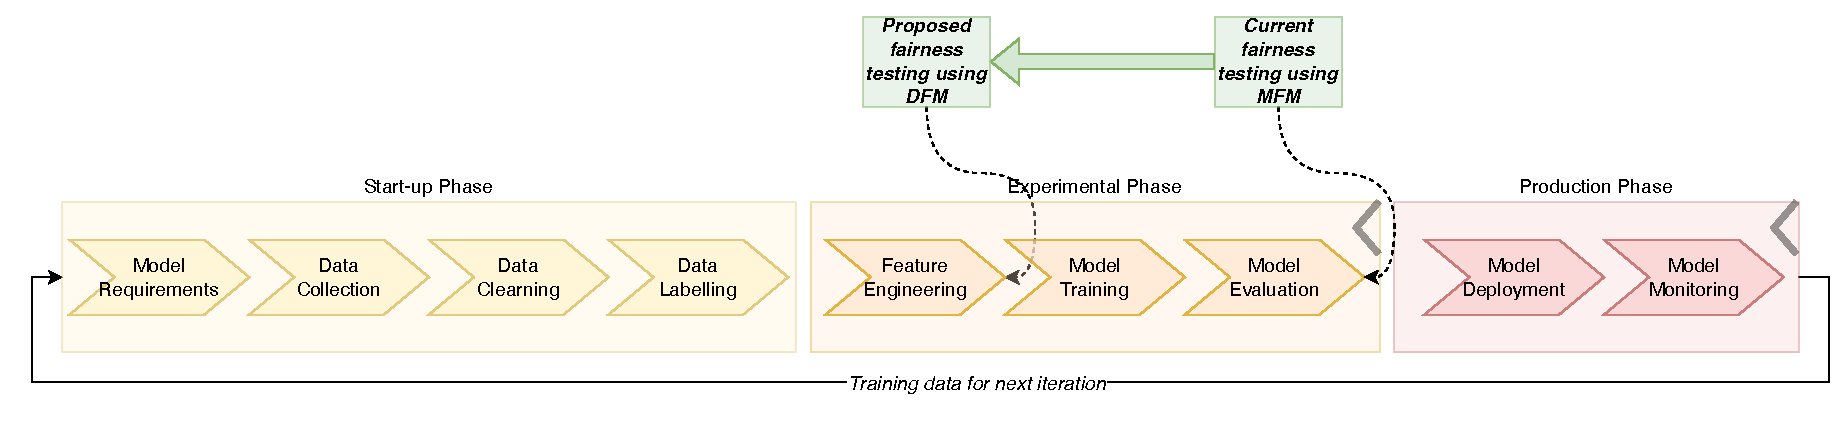
\includegraphics[width=\linewidth]{ml-lifecycle.pdf}
  \caption{Stages of the ML Lifecycle (adopted from
    \cite{amershi2019software,haakman2020ai,breck2019data}). Three
    distinct phases of the lifecycle are marked by different colours.
    Stages in the experimental and production phases may loop back to
    any prior stages, indicated by the large grey arrows. The location
    of fairness testing using DFM and MFM are marked by the green
    labels. The green arrow depicts the shift proposed by this study
    in ML fairness testing. }
  \label{fig:ml-lifecycle}
\end{figure*}

There is a growing consensus amongst academics that not all fairness
metrics can be satisfied simultaneously. There is also a consensus
that fairness and performance of ML systems are orthogonal to one
another and involve a trade-off. In fact, identifying the correct
fairness metric is the primary challenge which typically depends on
the domain and problem at hand. It is therefore recommended to
consider fairness as early as the requirements engineering and
software design
phase \cite{zhang2020machine,chen2022fairness,mehrabi2021survey,zhang2021ignorance}.

Several literature surveys have been conducted to classify and
catalogue various ML fairness testing and bias mitigation techniques.
\cite{wan2021modeling} conducted a large scale survey on
in-processing bias mitigation strategies and their effectiveness.
\cite{chen2022fairness} and \cite{mehrabi2021survey}
conducted a survey of existing literature on fairness testing in ML
systems. \cite{mehrabi2021survey} present a comprehensive survey
on the state-of-the-art research on fairness in ML with an emphasise
on fairness issues arising from both the data and the model.
\cite{chen2022fairness} survey 113 papers addressing fairness
testing and provide a formal definition of fairness bugs and fairness
testing in ML from a software engineering perspective. Authors also reflect on how
fairness testing differs from traditional software testing and provide
practical guidelines on how and where to test for fairness within the
entire Software Development
Lifecycle \cite{wan2021modeling,chen2022fairness,mehrabi2021survey}.

Prior work has also focused on conducting empirical analysis of bias
mitigation techniques. \cite{biswas2021fair} take a holistic
view of the entire ML pipeline and analyse the effect of common data
pre-processing techniques such as standardisation, feature selection,
encoding and sampling on the fairness of ML models. The analysis is
conducted using 37 real-world ML pipelines from Kaggle notebooks which
operate on five datasets. Typically data for the unprivileged group
tends to be limited which make pre and post processing bias mitigation
techniques less effective. \cite{feffer2022empirical} thus
conduct an empirical analysis of bias mitigation in combination with
popular ensemble techniques to understand the effectiveness of such
combinations. \cite{zhang2021ignorance} studied the effect of
training sample and feature sample size on the fairness of ML
models. Authors observe that a large feature sample combined with
a small training set helps reduce
bias \cite{biswas2021fair,feffer2022empirical,zhang2021ignorance}.

Prior work discussed so far operate under the assumption that the
training data and learning algorithm are accessible to the ML
practitioner---often referred to as \emph{white-box testing}. In
contrast, \emph{black-box testing} makes no such assumptions and
treats the entire ML pipeline as a black-box where we can only control
the input to the system and see the corresponding output. For such
situations, several test input generation techniques have been
proposed. \cite{galhotra2017fairness} proposed \emph{Themis},
a tool which automatically generates a testing suite to measure
discrimination in software using causal fairness
testing. \cite{udeshi2018automated} propose \emph{Aequitas}, an
automated tool that accepts a model and the protected attributes as
input and explores the input space to detect specific examples that
may produce discriminatory behaviour in the
model. \cite{aggarwal2019black} propose a new technique for
generating test input using symbolic execution which accounts for
correlation amongst the protected and unprotected
attributes \cite{aggarwal2019black,udeshi2018automated,galhotra2017fairness}.

This study conducts an empirical analysis of the relationship between
DFM and MFM, and as such, operates under white-box testing
assumptions. The experimental design of this study is similar in
spirit to that proposed by \cite{zhang2021ignorance}. However
our objective, results and implications are entirely different. While
\cite{zhang2021ignorance} study the effect of training and
feature sample size on the fairness of the model, this study aims to
understand the relationship between DFM and MFM. We analyse how change
in the distribution, sample size and number of features in the
training set affects this relationship. Through this analysis, we hope
to establish the role of DFM within the existing ML development
lifecycle.

\subsection{Machine Learning Lifecycle and Fairness
  Testing}\label{sec:ml-lifecycle}

Figure \ref{fig:ml-lifecycle} presents an overview of the various
stages of the ML lifecycle adapted from prior scientific literature.
The stages can be classified into three distinct phases as depicted by
the different colours. Although the figure presents a linear flow
amongst the various phases of the lifecycle, there are often several
feedback loops that may influence one another. The experimental and
production phases are marked with a gray arrow in the top right corner
as any stage in these phases can loop back to any prior stage in the
lifecycle \cite{amershi2019software,haakman2020ai,breck2019data}.

The upstream stages in the start-up phase tend to be ``data-centric''.
ML projects within the technology section typically work with
pre-existing data. However, in the recent shift towards application of
ML to safety critical domains, the ground truth must be established
through data collection, cleaning and
labelling \cite{sambasivan2021everyone,bosch2021engineering,amershi2019software}.

With the data ready, a highly experimental phase begins. This phase
involves several iterations to identify and engineer important data
features that boost the performance of the ML model. Historically, the
performance of ML models has been based on functional properties such
as the correctness and model relevance. However, in recent years,
non-functional properties such as robustness, fairness, security and
explainability have also been included \cite{zhang2020machine}.

The finalised model is deployed in a production environment to make
predictions on unseen data. ML systems---unlike traditional software
systems---do not fail explicitly in case of an error. But continue to
operate, albeit with a degraded performance. Since the output of the
ML model may be utilised by other software systems, the health of
production ML systems are continually monitored. Data will constantly
evolve and change as a reflection of the real world. However, ML
models are trained and tested using historical data which become
``stale'' after a certain period of time. Once the performance of the
live ML model drops below a pre-defined threshold, a new
training-testing-deployment cycle is issued. The next batch of
training data is typically derived by combining the unlabelled data in
production with the predictions of the live
model \cite{breck2019data,hynes2017data,breck2017ml}.

The status quo in ML fairness testing is to test for fairness after
the model has been trained, using the predictions of the model. In
this study, we wish to understand the benefits and limitations of
evaluating fairness prior to model training. This proposed shift in ML
fairness testing is marked by the green arrow in
Figure \ref{fig:ml-lifecycle}.

\section{Experimental Design}\label{sec:method}

\begin{figure*}
  \centering
  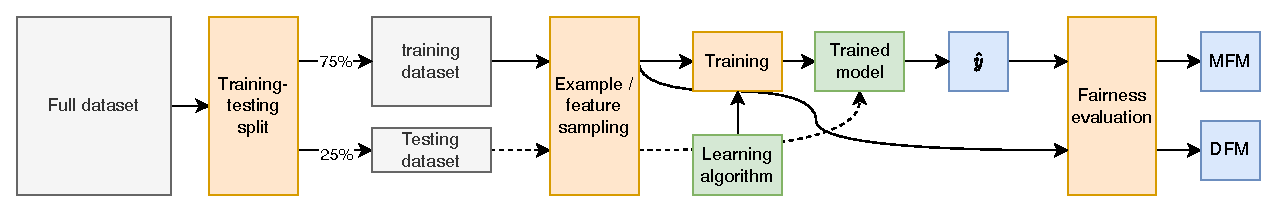
\includegraphics[width=\linewidth]{method.pdf}
  \caption{Methodology for evaluating fairness of datasets and ML
  models using DFM and MFM.}
  \label{fig:method}
\end{figure*}

This section presents details regarding the experimental design of
this study. The datasets, ML models and fairness metrics used in this
study are mentioned and the methodology used to evaluate DFM and MFM
is presented (summarised in Figure \ref{fig:method}). The section
concludes with an analysis of the experimental data collected in this
study.

\subsection{Datasets, ML Models and Fairness Metrics}\label{sec:method-parameters}

\begin{table}
  \centering
  \caption{Fairness metrics used in the study}
  \begin{tabular}{l r}
    \hline
    \textbf{\emph{DFM}}\\
    \hline
    DI & \(\displaystyle \frac{P(Y=1|D=0)}{P(Y=1|D=1)}\)\\
    SPD & \(\displaystyle P(Y=1|D=0)-P(Y=1|D=1)\)\\
    \hline
    \textbf{\emph{MFM}}\\
    \hline
    DI & \(\displaystyle \frac{P(\hat{Y}=1|D=0)}{P(\hat{Y}=1|D=1)}\)\\
    SPD & \(\displaystyle P(\hat{Y}=1|D=0)-P(\hat{Y}=1|D=1)\)\\
    \hline
  \end{tabular}
  \label{tab:fairness-metrics}
\end{table}

Table \ref{tab:fairness-metrics} shows the group fairness metrics
along with their mathematical formulas used in this study. We include
all group fairness metrics---namely \emph{Disparate Impact (DI)} and
\emph{Statistical Parity Difference (SPD)}---for which both model
dependent and independent variants are available. The DFM use the
labels of the data ($Y$) where as the MFM use the predictions of the
trained ML models ($\hat{Y}$). Favourable and unfavourable outcomes
are represented by $1$ and $0$ respectively. Similarly, privileged and
unprivileged groups of the protected attribute ($D$) are represented
by $1$ and $0$ respectively. All fairness metrics and datasets used in
this study are obtained from the \emph{AIF360} python
library \cite{bellamy2019ai}.

\begin{table}
  \centering
  \caption{Datasets used in the study}
  \begin{tabular}{l l r}
    \hline
    \textbf{Name} & \textbf{Prot.} & \textbf{\#Eg.}\\
    \hline
    German \cite{hofmann1994german} & age, sex & 1000\\
    Compas\cite{angwin2016machine} & race, sex & 6167\\
    MEPS \cite{mepsdata} & race & 15675\\
    Bank\cite{moro2014data} & age & 30488\\
    Adult\cite{kohavi1996scaling} & race, sex & 45222\\
    \hline
  \end{tabular}
  \label{tab:datasets}
\end{table}

Table \ref{tab:datasets} presents the datasets used in this study. We
consider tabular datasets which have been extensively used in prior
scientific contributions on ML fairness
testing \cite{zhang2021ignorance,biswas2020machine,biswas2021fair,chen2022fairness}. Based
on prior work, we only consider one protected attribute at any given
time thus giving us eight independent datasets. We follow the default
pre-processing steps implemented in the AIF360 library---missing
values are dropped and categorical features are label encoded. Prior
to training, the features in the training and testing subsets are
standardised by removing the mean of the sample and scaling to unit
variance.

We use the scikit-learn \cite{pedregosa2011scikit} python library for
creating the train-test splits and training the ML models. We use four
ML models of varying complexity namely, \emph{Logistic Regression},
\emph{Decision Trees}, \emph{Random Forest} and \emph{Ada boost} based
on their popularity in practise and in prior scientific
publications \cite{zhang2021ignorance,biswas2021fair,biswas2020machine}.

\subsection{Fairness Evaluation}\label{sec:method-fair-eval}

\begin{table}
  \centering
  \caption{Parameters of the study}
  \begin{tabular}{l r}
    \hline
    \textbf{Parameter} & \textbf{Count}\\
    \hline
    Fairness metrics & $2$\\
    ML models & $4$\\
    Datasets & $8$\\
    Total cases & $8\times4=32$\\
    Iterations & $50$\\
    Total fairness evaluation cycles & $32\times50=1600$\\
    \hline
  \end{tabular}
  \label{tab:parameters}
\end{table}

Figure \ref{fig:method} presents the methodology used in this study
for evaluating the fairness of ML models and datasets. A 75--25 split
with shuffling is used to create the training and testing splits. DFMs
and MFMs are used to quantify the bias in the underlying distribution
of the training set and the predictions of the models respectively. We
adopted the transformation steps from prior work to scale all fairness
metric values between $0$ and $1$ such that higher values indicate
more bias \cite{zhang2021ignorance,hort2021fairea}.

We extend the above experiment further in two ways. First, we
experiment with different number of examples and second with different
number of features in the training set. For both experiments, we
shuffle the order of the examples in the training and testing sets.
Additionally, for the feature sample size experiment we shuffle the
order of the features.

For the training sample size experiment, we generate different
training samples of varying sizes starting from 10\% of the original
training data, and increase in steps of 10\% until the full quantity
is reached. For the feature sample size experiment, we start with
a minimum of three features (in addition to the protected attribute
and target) and introduce one new feature until all the features are
utilised. Both the training and testing sets undergo the same feature
sampling procedure in the feature sample size experiment. No such
sampling is done in the testing set for the training sample size
experiment.

Table \ref{tab:parameters} summarises the parameters of the study. We
train 4 ML models on 8 datasets producing 32 total cases. The fairness
for each case is evaluated 50 times using two fairness metrics, thus
producing a total of 1600 training and fairness evaluation cycles.

\subsection{Correlation Analysis}\label{sec:corr-analysis}
%% !TODO add a table with clear interpretation of correlation results;
%% consult notes for details

We use correlation analysis to study the relationship between DFM and
MFM with-respect-to change in three experimental
factors---distribution, size and features of the training set.
Spearman Rank Correlation is used to quantify the linear relationship
between the DFM and MFM since it does not assume normality and is
robust to outliers. We repeat all experiments 50 times and report the
statistical significance of our results. We consider cases where
$pvalue\le0.05$ to be statistically significant in our evaluation.

We do not apply the \emph{Bonferroni correction} to the correlation
analysis results. Although we report the $pvalue$ for completeness, we
do not base our implications only on the statistically significant
results. But rather on general trends observed in our analysis.

A positive correlation means that the DFM and MFM changed in the same
direction and thus \emph{convey the same information}. A positive
correlation indicates that both the DFM and MFM show presence of bias
in the training data and in the model predictions respectively.

A negative correlation between the DFM and MFM means that they changed
in the opposite direction and \emph{do not convey the same
information}. This indicates that the bias in the model predictions
was lower than that present in the training data. Note that the
opposite event---of bias in the model predictions being higher than
that present in the training data---is unlikely to occur. ML models
cannot manifest bias towards a particular protected group if the
training data is unbiased to begin with.

The implications of the correlation results varies based on the
experimental factor. A detailed discussion is presented in the
corresponding sub-sections of Section \ref{sec:implications}.

\subsection{Distribution of Experimental Data}\label{sec:data-analysis}

\begin{figure}
  \centering
  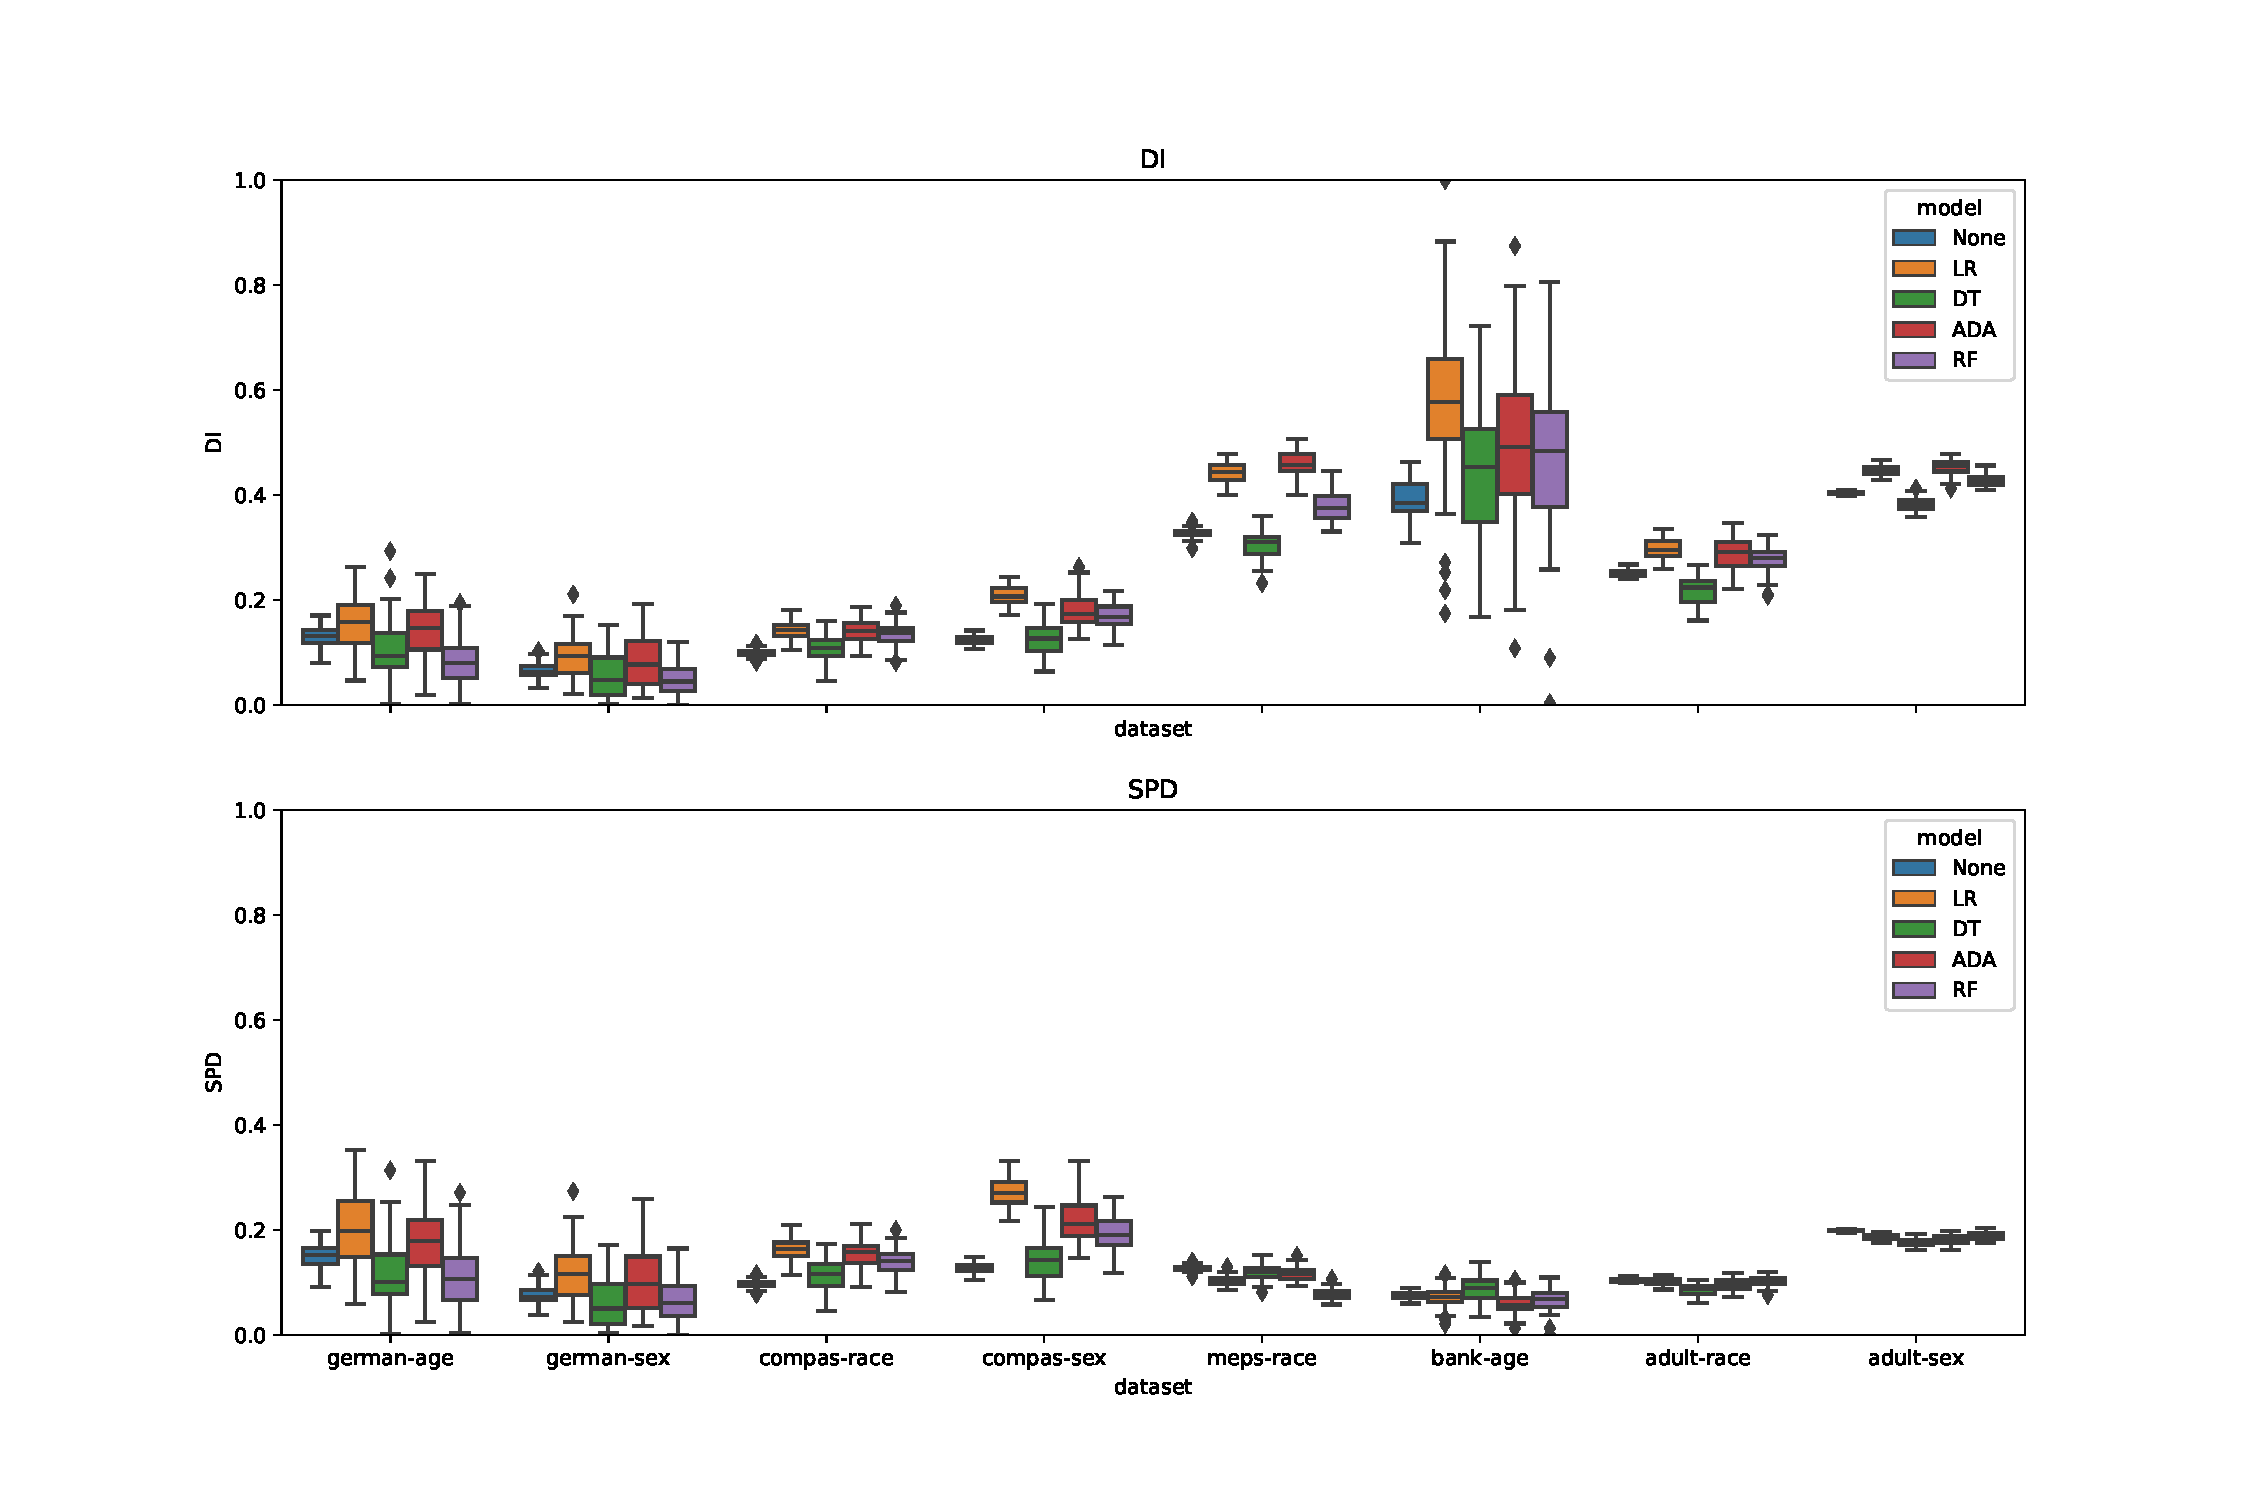
\includegraphics[width=\linewidth]{boxplot--dataset--di-spd--exp-full.pdf}
  \caption{Boxplot showing distribution of DFM and MFM for all
    datasets, models and fairness metrics.}
  \label{fig:boxplot--dataset--di-spd--exp-full}
\end{figure}

Figure \ref{fig:boxplot--dataset--di-spd--exp-full} presents a boxplot
with the distribution of DFM and MFM for all datasets, models and
fairness metrics. The x-axis represents the datasets used in this
study while the y-axis presents the value of the fairness metric. The
models used in this study are represented using different
colours---note that the model ``None'' represented in blue refers to
the DFM. Both the fairness metrics DI (top) and SPD (bottom) are
presented in separate plots.

Comparing the boxplots for DI and SDP, we note that they follow a
similar pattern of distribution. Comparing the DFM and MFM for any
given ML model and dataset, we observe a difference in the
distribution of the DFM and MFM. In several instances the tree-based
classifiers (DT and RF) make fairer decisions compared to the other
classifiers, sometimes even better than the baseline provided by the
DFM.

The variability of MFM tends to be higher than DFM. This is because,
in addition to the randomness from the data shuffling in the training
set, the models are assigned random initial states in every iteration
thus resulting in different predictions across the iterations and
consequently varying MFM values.

\section{Results}\label{sec:results}

This section presents the analysis of the relationship between DFM and
MFM. We use correlation to evaluate the relationship between DFM and
MFM with-respect-to three experimental factors: distribution, size and
features of the training set (see Section \ref{sec:corr-analysis} for
interpretation of correlation analysis and how it is used in this
study). This section is broken further into three subsections based on
the research questions.

\subsection{RQ1. What is the relationship between DFM and MFM as
the fairness properties of the underlying training dataset
changes?}\label{sec:results-full-rel}

\begin{figure}
  \centering
  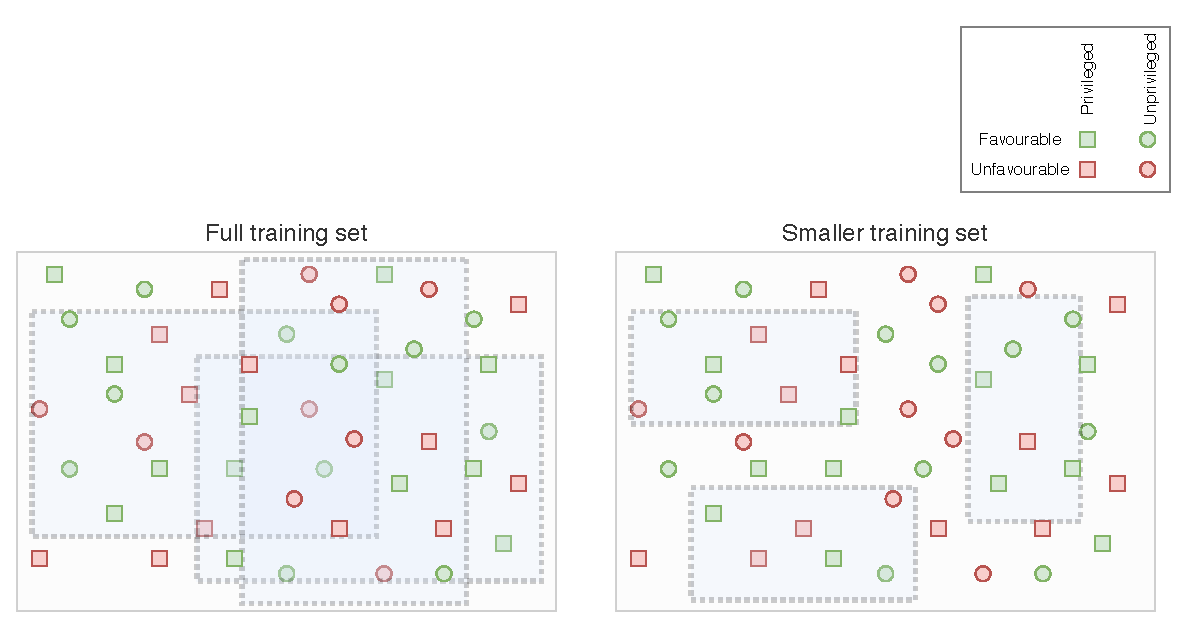
\includegraphics[width=\linewidth]{shuffle.pdf}
  \caption{Visual explanation of rationale for using smaller training
    sample to simulate change in the distribution of the training
    data. The grey boxes represent the full dataset while the blue
    boxes represent the training set for three hypothetical
    iterations. More overlap in the blue boxes depicts less
    distribution change and vice-versa.}
  \label{fig:shuffle}
\end{figure}

\begin{figure}
  \centering
  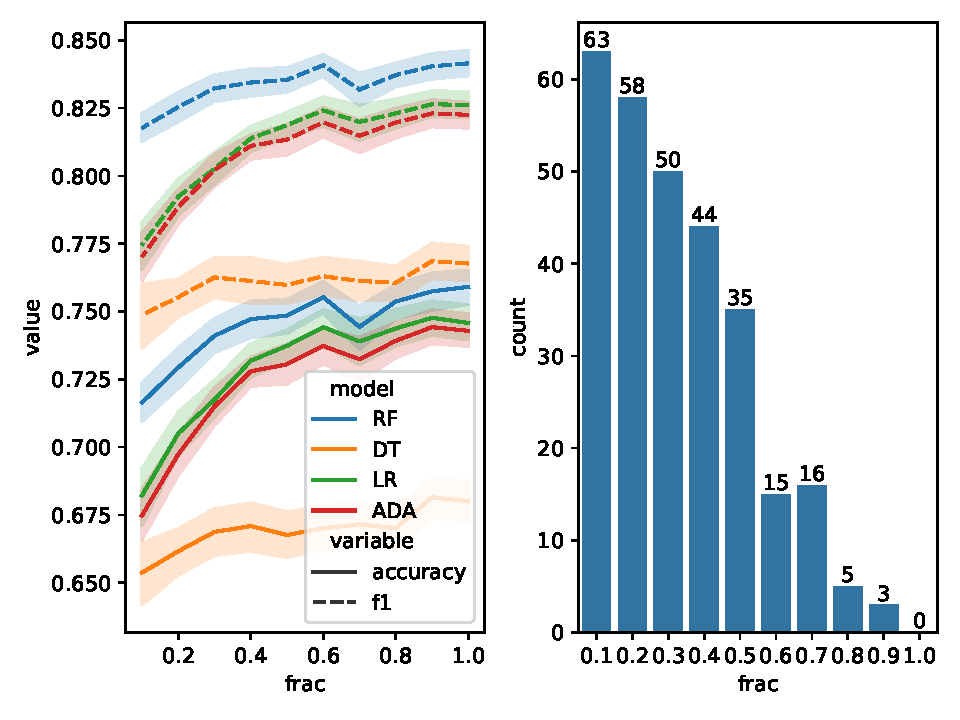
\includegraphics[width=\linewidth]{training-set-frac-threshold.pdf}
  \caption{\emph{\textbf{(left)}} Lineplot showing relationship
    between performance metrics and training sample size in the
    \emph{german-age} dataset. Data from the 50 iterations is
    aggregated using the mean, the error bars show the standard
    deviation. \emph{\textbf{(right)}} Countplot showing number of
    cases with significant change in accuracy and f1 when trained
    using the full vs. smaller training sample size.}
  \label{fig:training-set-frac-threshold}
\end{figure}

\begin{figure}
  \centering
  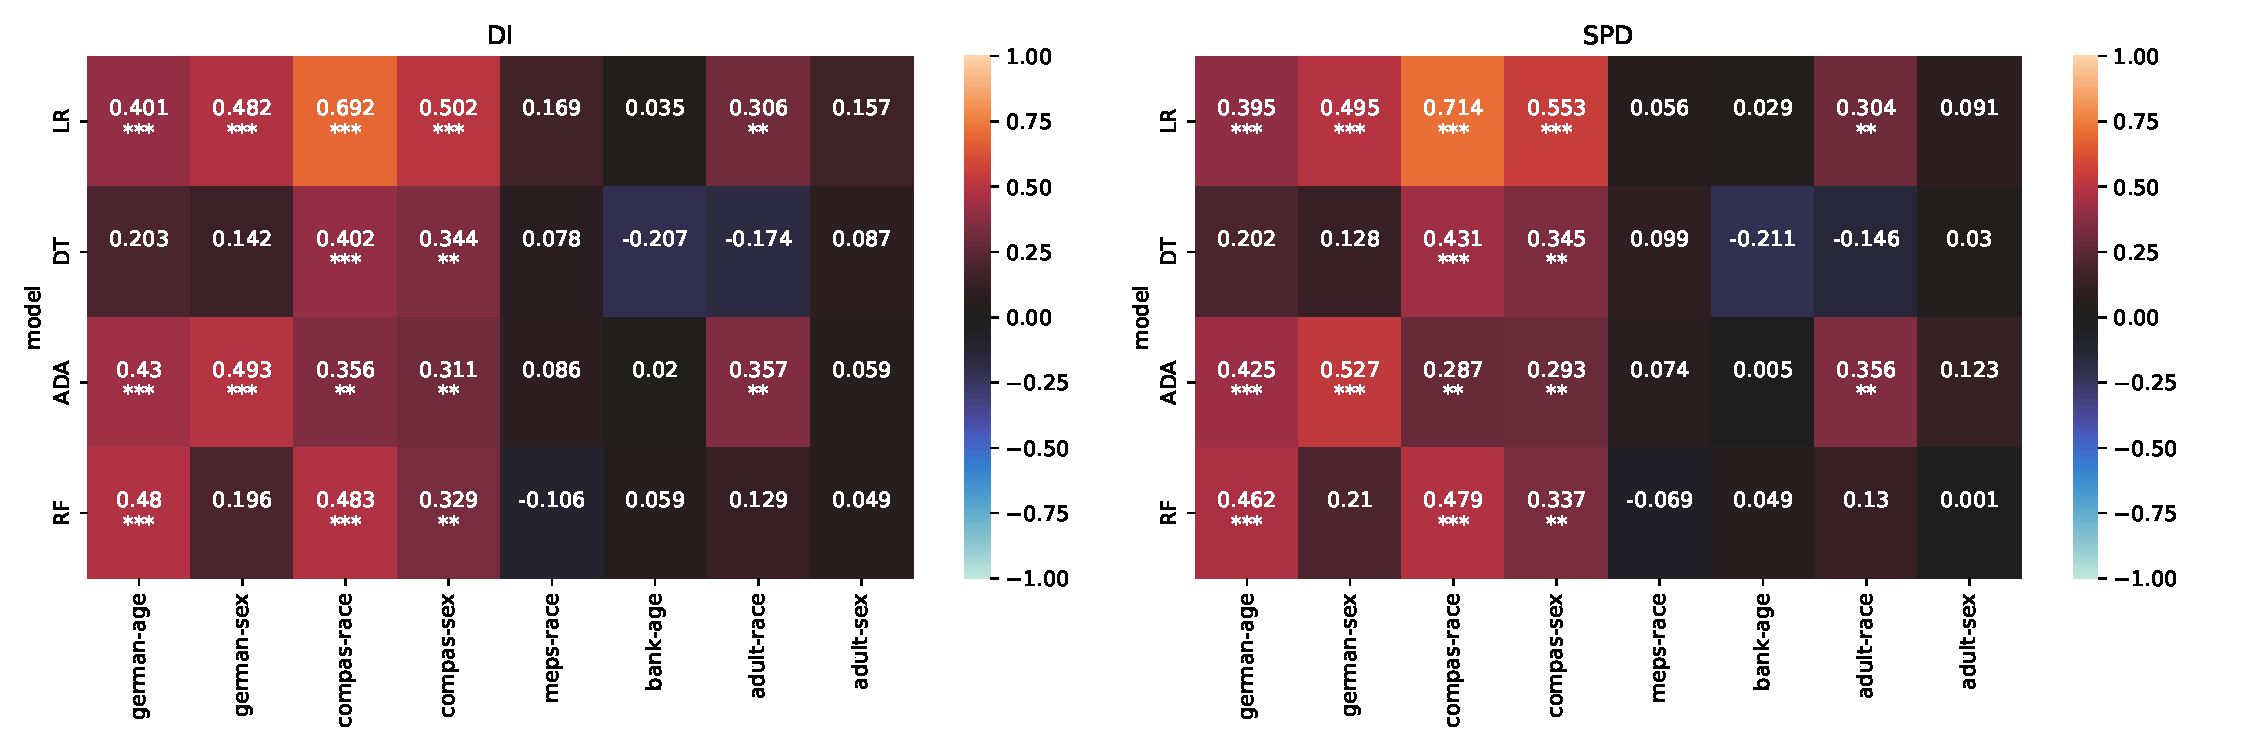
\includegraphics[width=\linewidth]{heatmap--corr--training-sets-frac.pdf}
  \caption{Heatmap showing correlation between DFM and MFM for all
    models and datasets using training data with simulated
    distribution change. Each block is representative of 50
    iterations. The statistically significant cases are marked with an
    asterisks. We primarily observe bright hues of red indicating that
    the DFM and MFM convey the same information. This means that DFM
    can be used to identify fairness related data drifts in automated
    ML pipelines.}
  \label{fig:heatmap--corr--training-sets-frac}
\end{figure}

\begin{figure}
  \centering
  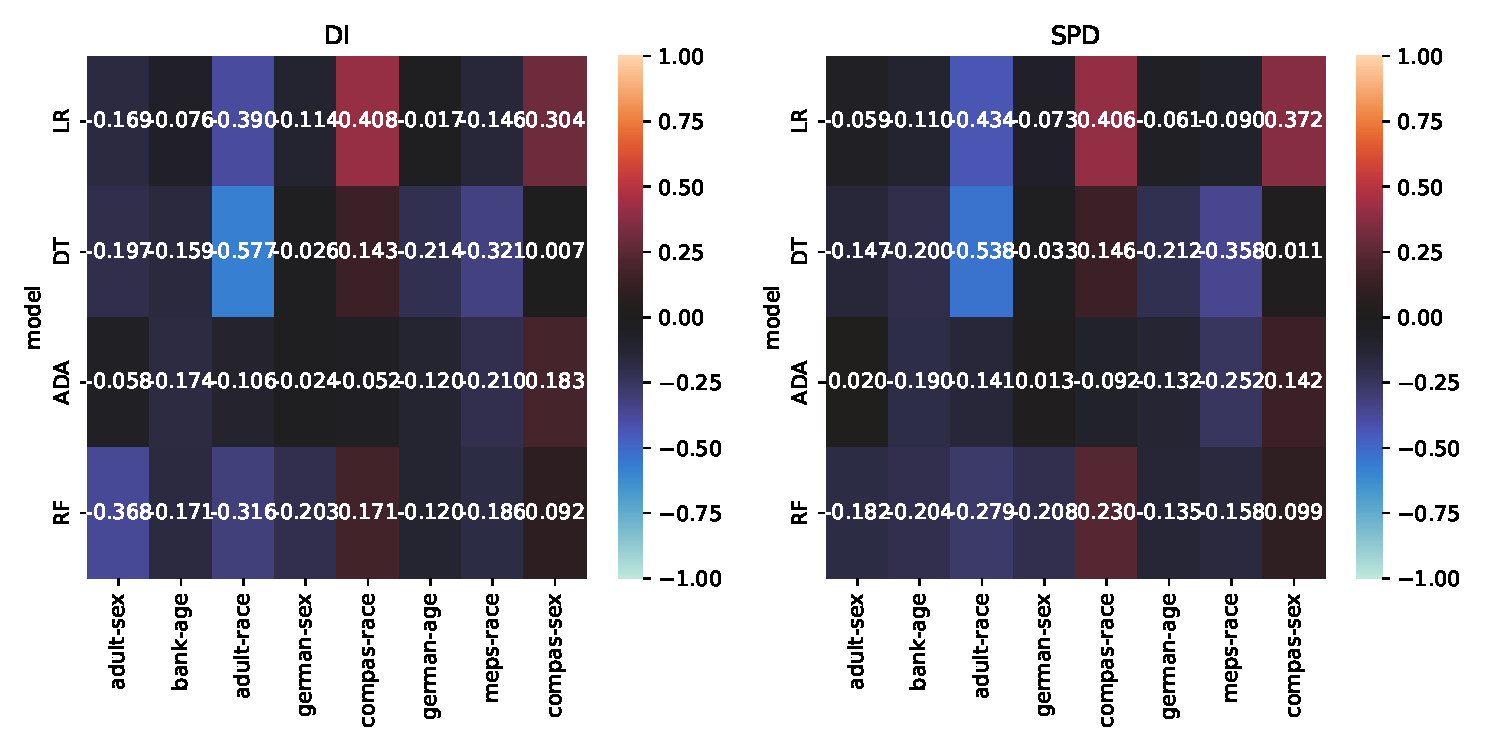
\includegraphics[width=\linewidth]{heatmap--corr--full-data.pdf}
  \caption{Heatmap showing correlation between DFM and MFM using
    training data without significant distribution change. Each block
    is representative of 50 iterations. In contrast to
    Figure \ref{fig:heatmap--corr--training-sets-frac}, we primarily
    observe darker colours indicating that the DFM and MFM no longer
    convey the same information.}
  \label{fig:heatmap--corr--full-data}
\end{figure}

To simulate change in the distribution of the training data, we use a
smaller subset of the original training data. Figure \ref{fig:shuffle}
visually motivates this approach. Privileged examples ($D=1$) are
represented using squares while unprivileged examples ($D=0$) are
represented using circular points. The label of the examples are
represented using colour---green for favourable ($Y=1$) and red for
unfavourable ($Y=0$) examples. The large grey boxes represent the
original dataset while the blue boxes represent the training dataset.

The figures present three hypothetical iterations of the data sampling
process to create the training set. The left figure presents the
scenario where the full training set is used while the right figure
presents the scenario where a smaller portion of the full training set
is used. As seen from the figure, there is more overlap amongst the
examples in the full training set in every iteration. In contrast,
there is less overlap amongst the examples in the smaller training
set. The distribution in smaller training samples will thus change
more frequently in the 50 iterations and capture a wide variety of
data fairness properties.

The data quality in smaller training samples will however deteriorate.
To identify a sample size that captures a variety of data fairness
properties while also being a realistic training dataset, we analyse
the \emph{accuracy} and \emph{f1 score} of the models across different
training sample sizes (as explained in
Section \ref{sec:method-fair-eval}). Next, we conduct \emph{student
t-test} to identify the smallest sample size where the performance of
the models is similar to that obtained when trained using the full
training set.

Figure \ref{fig:training-set-frac-threshold} (right) presents a
histogram of the number of cases where there was a significant
difference between the two populations. We note that there is a
significant difference in the performance of the models, in the
majority of the cases when the training size is reduced to 50\%. The
performance however remains consistent when using a training size of
60\% or higher. This is also corroborated by the lineplot in
Figure \ref{fig:training-set-frac-threshold} (left) which shows the
accuracy and f1 of all models across various training sample sizes in
the \emph{german-age} dataset. We observe that the performance
stabilises starting from 60\% training sample size. Thus for the
majority of the cases, a training sample of 60\% allows us to train
models with acceptable performance, while also capturing a wide
variety of fairness issues in the underlying training data within the
50 iterations.

Figure \ref{fig:heatmap--corr--training-sets-frac} shows the
correlation between the DFM and MFM across all models and datasets
when trained using data with simulated distribution change as outlined
above. The models used in this study are represented along the y-axis
and the datasets along the x-axis. Darker colours indicate weaker
correlation whereas brighter colours indicate stronger correlation.
Positive correlation is indicated using hues of red while negative
correlation is indicated using hues of blue. The correlation between
DFM and MFM for both fairness metrics are shown separately. We
primarily observe a positive correlation between the DFM and MFM. This
indicates that the DFM and the MFM convey the same information as the
distribution---and consequently the fairness properties---of the
underlying training dataset changes.

In contrast to Figure \ref{fig:heatmap--corr--training-sets-frac},
Figure \ref{fig:heatmap--corr--full-data} shows the correlation
between DFM and MFM when trained using data without sufficient
distribution change. Due to lack of significant change in the
distribution of the training data, we primarily observe darker colours
indicating that the DFM and MFM are not linearly related to one
another anymore.

\highlight{\textbf{Answer to RQ1:} DFM and MFM are positively
correlated and thus convey the same information as the
distribution---and consequently the fairness properties---of the
underlying training dataset changes.}

\subsection{RQ2. How does the training sample size affect the
correlation between DFM and MFM?}\label{sec:results-corr-frac}

\begin{figure}
  \centering
  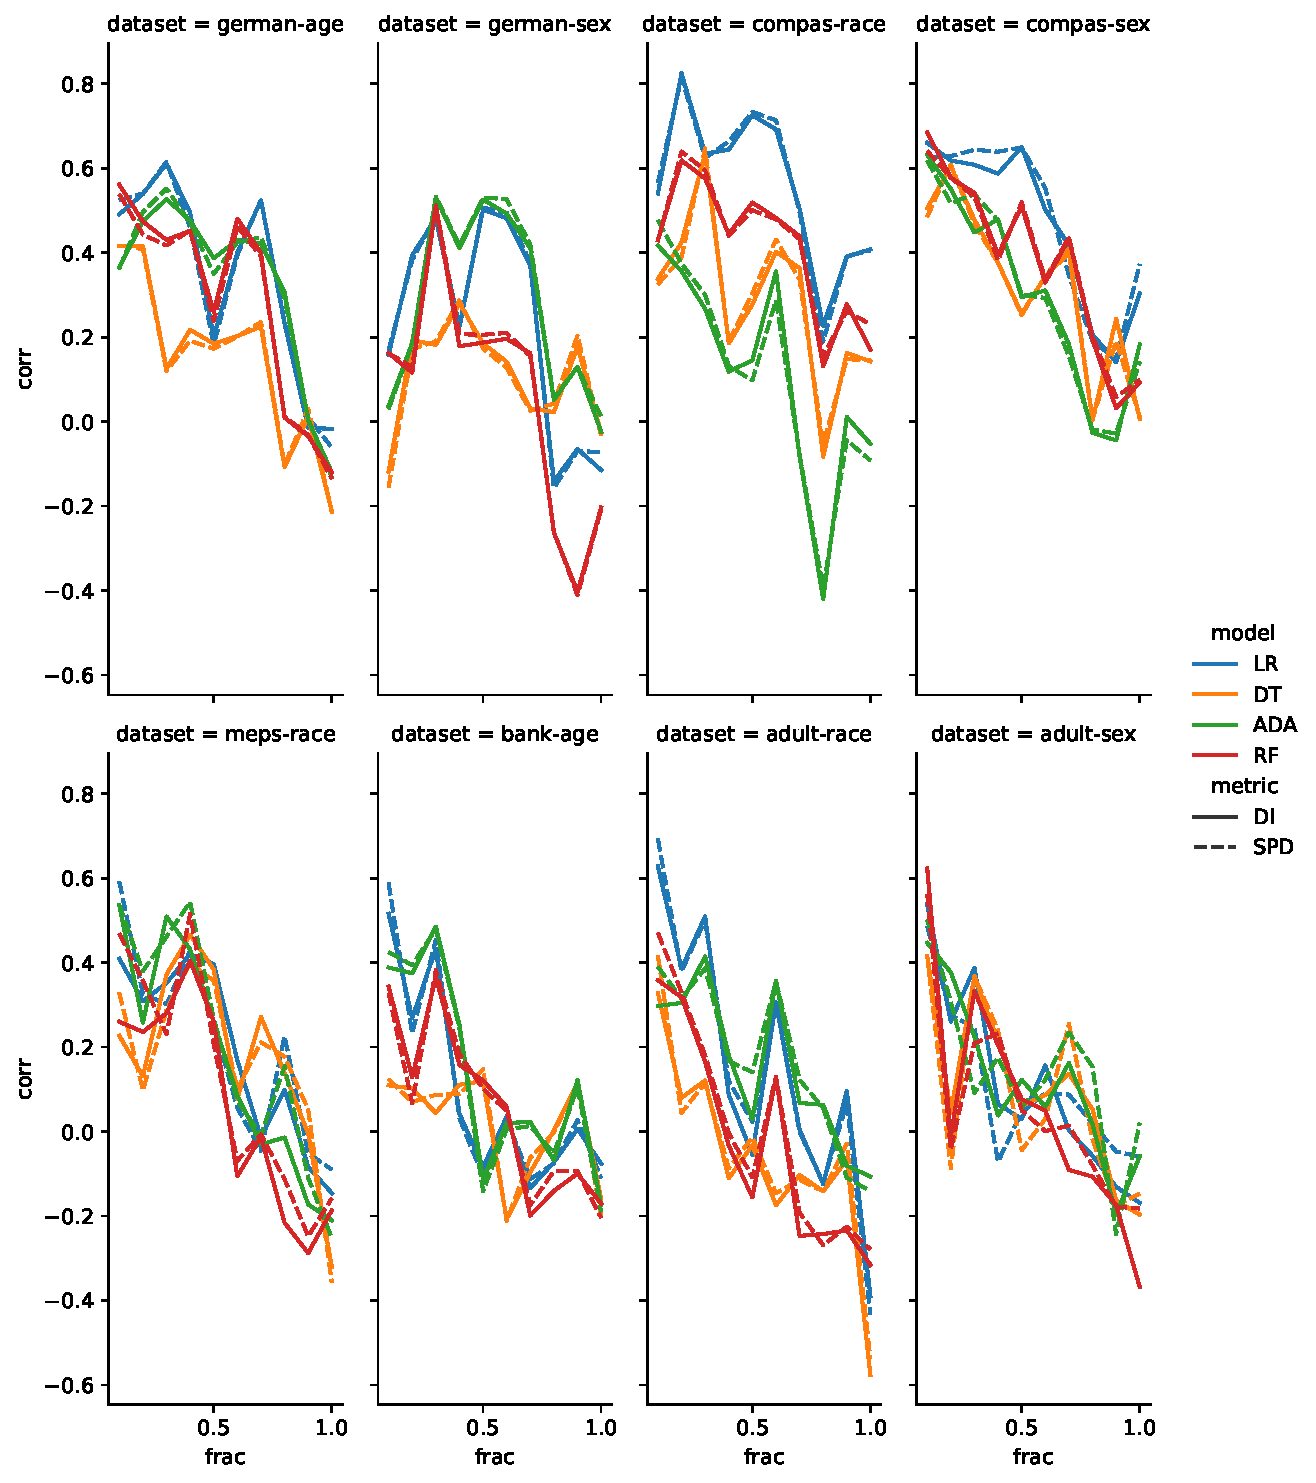
\includegraphics[width=\linewidth]{lineplot--frac--corr.pdf}
  \caption{Lineplot showing relationship of correlation (between DFM
    and MFM) with training sample size for all datasets and models.
    Data from the 50 iterations is aggregated using the mean value.
    The correlation decreases as the training sample size is
    increased. This indicates that with sufficient training data, ML
    models are able to circumvent some of the bias in the underlying
    training set.}
  \label{fig:lineplot--frac--corr}
\end{figure}

In Figure \ref{fig:heatmap--corr--training-sets-frac}, the correlation
in the smaller datasets are more positive compared to the larger
datasets when trained using a smaller training sample size. When the
training sample size is increased, the correlation in the datasets
decrease as observed in Figure \ref{fig:heatmap--corr--full-data}.

Based on these observations, we hypothesise that the quantity of
training data influences the correlation between DFM and MFM. Our
hypothesis is corroborated by Figure \ref{fig:lineplot--frac--corr}
which shows the relationship of the correlation with various training
sample sizes, for all datasets and models. The x-axis presents the
training sample size and the y-axis presents the correlation between
the DFM and MFM. The colours represent the models while the style of
the line represents the two fairness metrics. Each dataset is shown as
a separate subplot. The overwhelming majority show that the
correlation between the DFM and MFM decreases as we increase the
training sample size.

\highlight{\textbf{Answer to RQ2:} The training sample size has
a profound effect on the relationship between the DFM and MFM. The
correlation between the DFM and MFM decreases as we increase the
training sample size.}

\subsection{RQ3. What is the relationship between DFM and MFM
across various training and feature sample
sizes?}\label{sec:results-size-feature-sample}

\begin{figure}
  \centering
  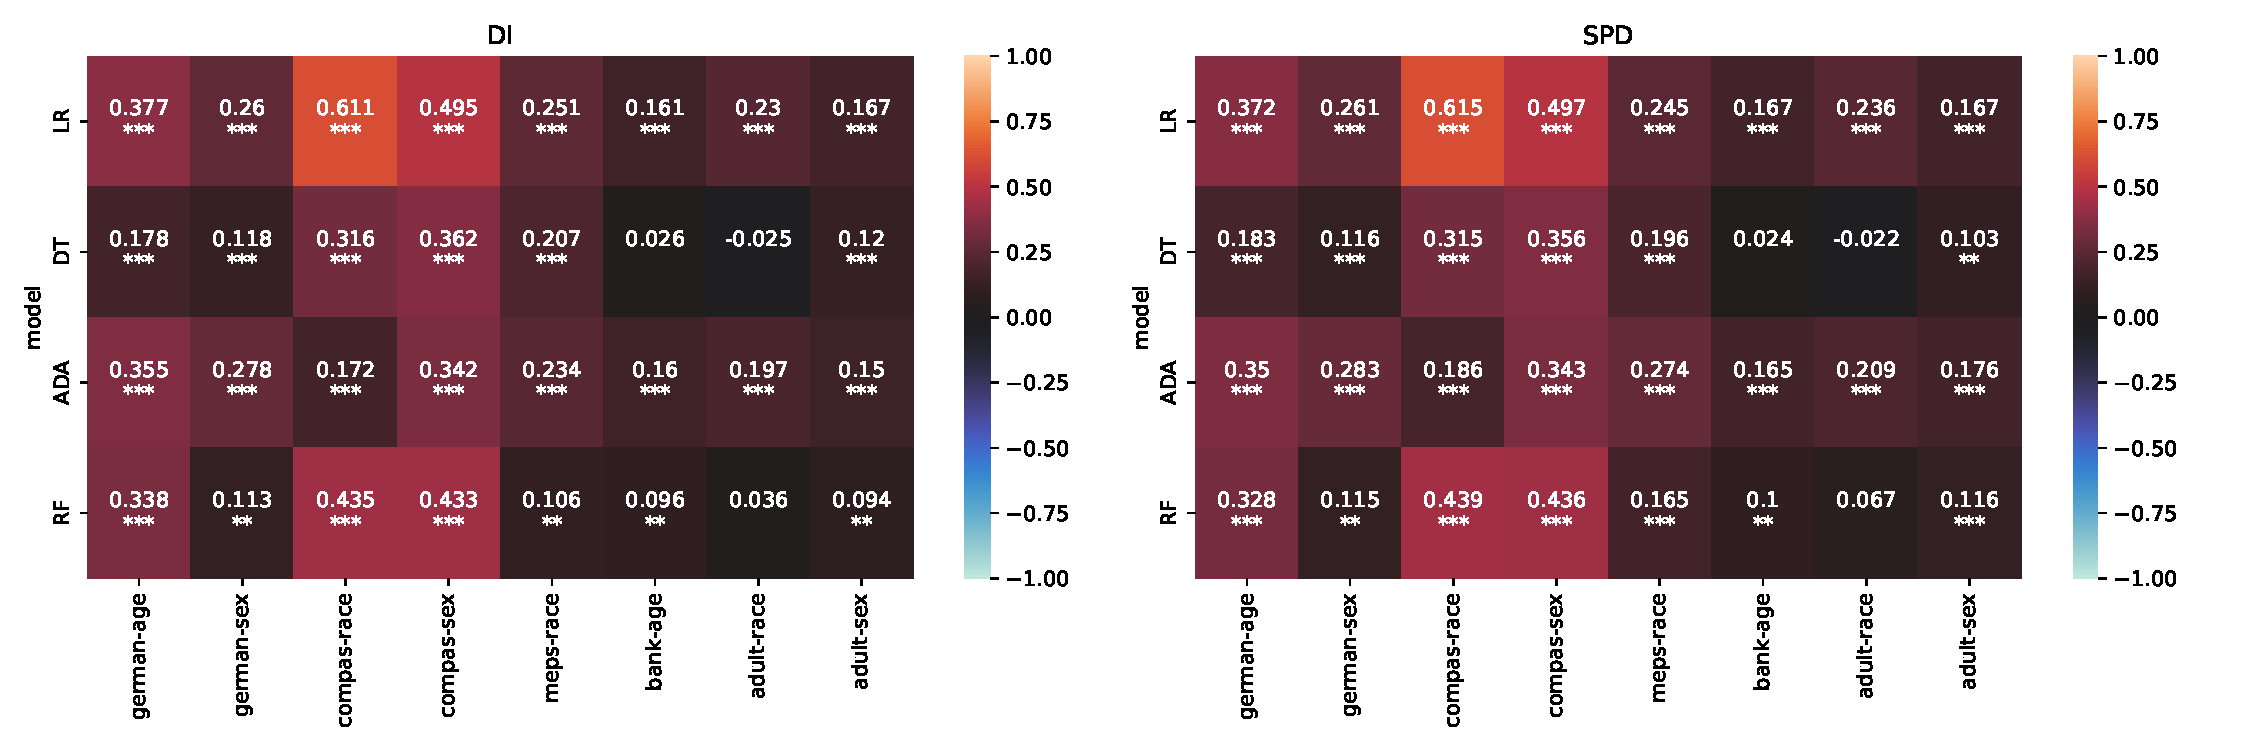
\includegraphics[width=\linewidth]{heatmap--corr--frac.pdf}
  \caption{Heatmap showing correlation between DFM and MFM across all
    training sample sizes. Each block is representative of 50
    iterations $\times$ 10 training sample size $=$ 500 data points.
    The statistically significant cases are marked with an asterisks.
    We primarily observe hues of red indicating that the DFM and MFM
    convey the same information. When experimenting with the training
    sample size, DFM can aid practitioners catch fairness issues
    upstream and avoid execution costs of a full training cycle.}
  \label{fig:heatmap--corr--frac}
\end{figure}

\begin{figure}
  \centering
  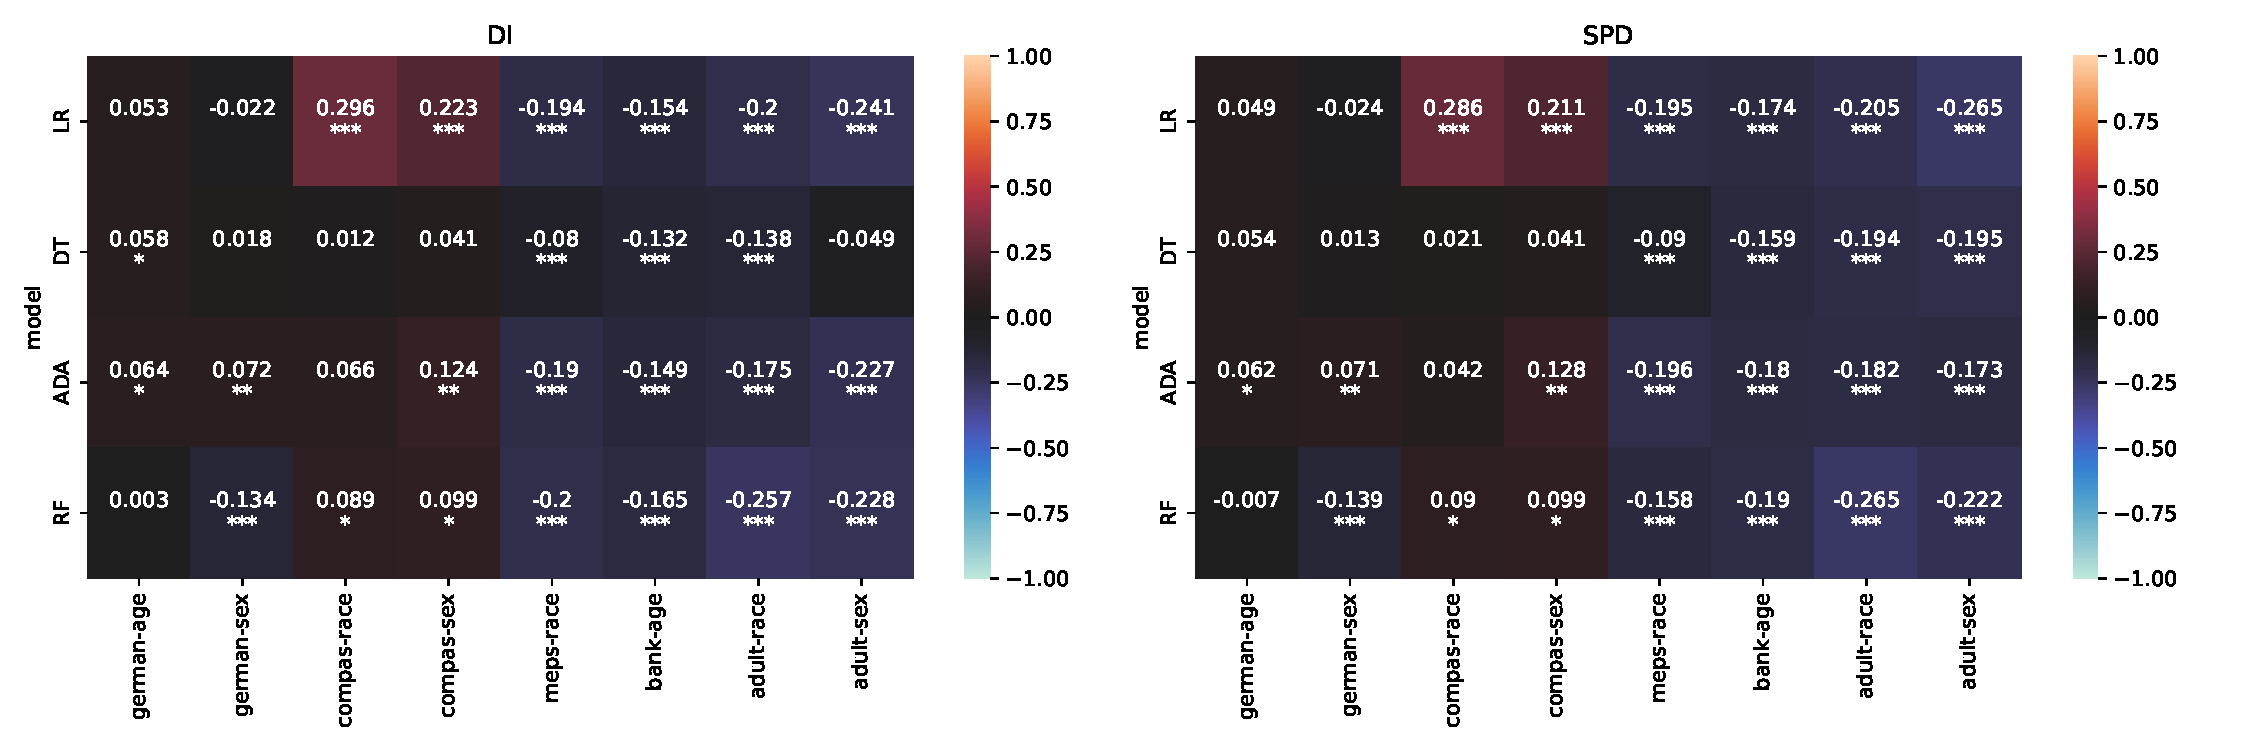
\includegraphics[width=\linewidth]{heatmap--corr--num-features.pdf}
  \caption{Heatmap showing correlation between DFM and MFM across
    various feature sample sizes. Each block is representative of data
    points from 50 iterations $\times$ the number of features in the
    dataset. We primarily observe darker colours indicating that the
    DFM and MFM do not convey the same information. When experimenting
    with the feature sample size, practitioners must test for fairness
    both before and after training.}

  \label{fig:heatmap--corr--num-features}
\end{figure}

\begin{figure}
  \centering
  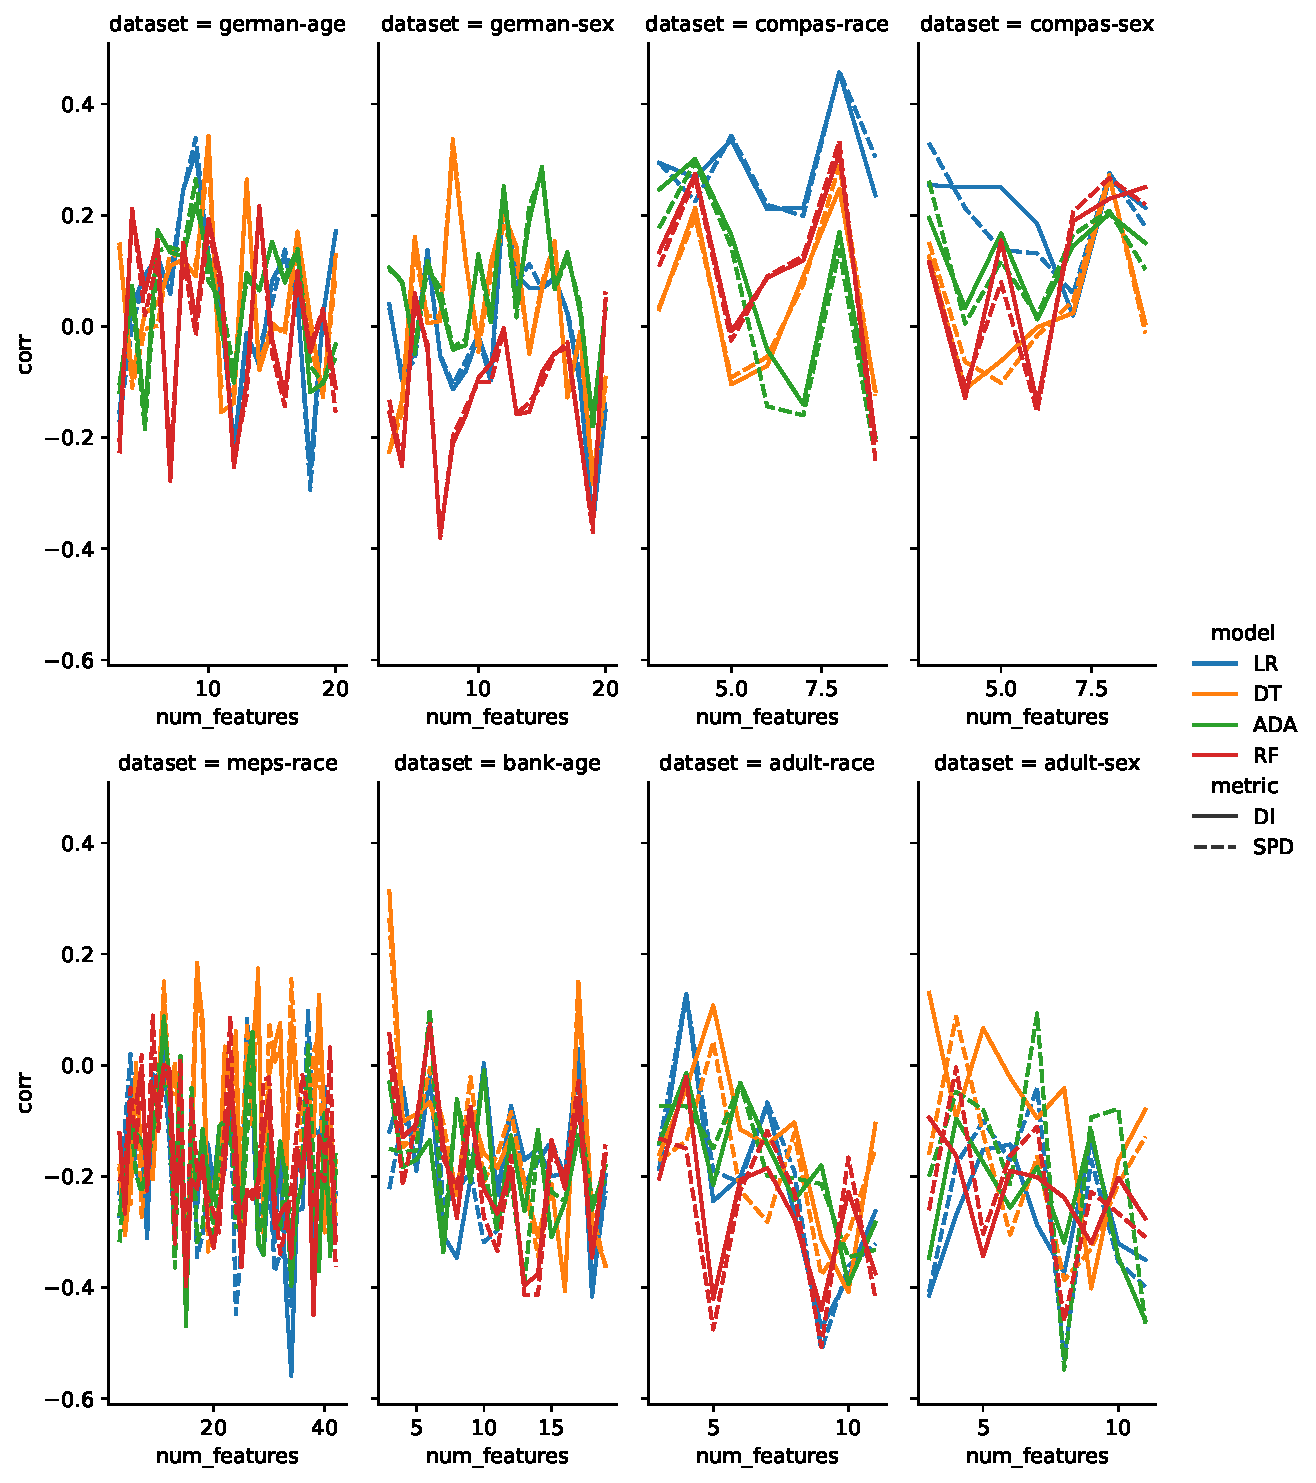
\includegraphics[width=\linewidth]{lineplot--num-features--corr.pdf}
  \caption{Lineplot showing relationship of correlation (between DFM
    and MFM) with feature sample size for all datasets and models.
    Data from the 50 iterations is aggregated using the mean value.
    There is no discernible relationship since the number of features
    does not influence the DFM.}
  \label{fig:lineplot--num-features--corr}
\end{figure}

\subsubsection{Training Sample Size}

In this section we analyse the relationship between DFM and MFM across
varying training sample sizes. In contrast to
Section \ref{sec:results-corr-frac} where we calculated the
correlation between DFM and MFM within each training sample size, here
we calculate the correlation across all training sample sizes. The
correlation between the DFM and MFM is shown in
Figure \ref{fig:heatmap--corr--frac}. We primarily observe colours
indicating that the DFM and MFM convey similar information as the
training sample size changes.

\subsubsection{Feature Sample Size}

In this section we analyse the relationship between the DFM and MFM
across varying feature sample sizes. In contrast to the training
sample size experiment above, we change the number of features in the
training set and randomise the feature order in each iteration.
Figure \ref{fig:heatmap--corr--num-features} presents the correlation
between the DFM and MFM across all feature sample sizes. We primarily
notice darker colours indicating that there is no significant
correlation between the DFM and MFM as the number of features in the
training dataset changes.

From Table \ref{tab:fairness-metrics}, we note that the feature sample
size does not affect the DFM thus explaining the lack of significant
correlation between the DFM and MFM. The larger datasets show a more
negative correlation. As explained in
Section \ref{sec:results-corr-frac}, this is because the larger
datasets have sufficient training data for the model to mitigate some
of the bias in the underlying training set. This can also be verified
in Figure \ref{fig:lineplot--num-features--corr} which shows the
relationship between the correlation and the feature sample sizes for
all datasets and models. There is no discernible relationship between
the correlation and the feature sample size in the top row containing
datasets which are smaller in size but contain a large number of
features. A slight relationship can only be observed in the bottom
right subplots which contain datasets which are larger in size but
contain less number of features.

\highlight{\textbf{Answer to RQ3:} DFM and MFM convey similar
information as the training sample size changes but not when the
feature sample size changes.}

\section{Implications}\label{sec:implications}
The implications of the results presented in Section \ref{sec:results}
are discussed in this section.

\subsection{Data Drift}\label{sec:discuss-data-drift}

Results from RQ1 indicate that the DFM and MFM convey the same
information when the distribution and consequently the fairness
properties of the training data changes. ML systems running in a
production environment are often monitored to detect degradation in
model performance. As shown in Figure \ref{fig:ml-lifecycle}, a
standard practise is to combine the data encountered by the model in
the production environment with its predictions to create the training
set for the next iteration \cite{biessmann2021automated}. Since data
reflects the real world, change in its underlying distribution over
time is eminent. Our results indicate that DFM can be used as a early
warning system to identify fairness related data drifts in automated
ML pipelines.

\subsection{Fairness, data size and correctness trade-off}\label{sec:discuss-fair-eff-perf-trade}

\begin{figure}
  \centering
  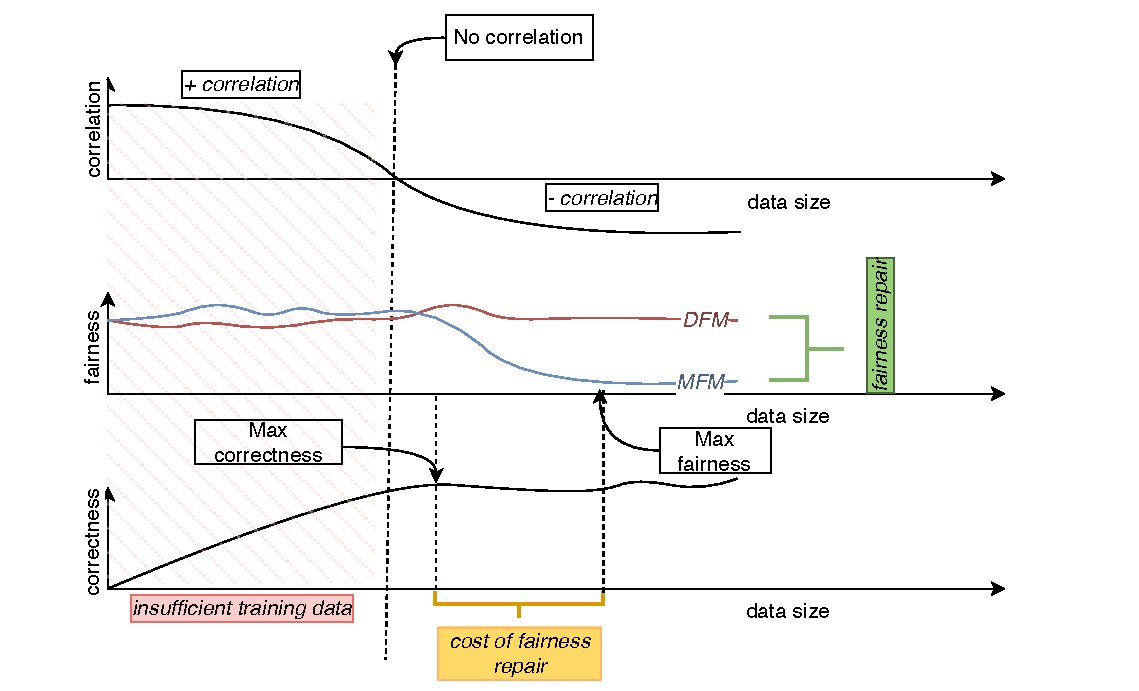
\includegraphics[width=\linewidth]{tradeoff.pdf}
  \caption{Visual representation of trade-offs between fairness, data
    size and correctness of ML models.}
  \label{fig:tradeoff}
\end{figure}

Results from RQ2 indicate that the quantity of training data
profoundly influences the relationship between DFM and MFM.
Figure \ref{fig:tradeoff} presents a visual explanation of the RQ2
results along with its implications to fairness and performance (or
correctness) of ML models. The top subplot visually summarises the RQ2
results observed in Figure \ref{fig:lineplot--frac--corr}. We
primarily see a positive correlation between the DFM and MFM in
smaller training sample sizes which indicates presence of bias in both
training data and model predictions. Thus a positive correlation
between the DFM and MFM may indicate lack of sufficient training data.
Under such circumstances, practitioners can either choose to collect
more data if possible or use bias mitigation techniques to address the
fairness issue.

% do we have proof of this claim?
The middle subplot depicts the effect of training sample size on DFM
and MFM. As the training data is increased, DFM remains consistent
while MFM reduces. Thus, with sufficient training data, the
correlation starts to drop and eventually becomes negative. This
indicates that the models learn to make fairer predictions and are
able to circumvent the bias in the training data to a certain extent.
A lower MFM value compared to DFM does not however guarantee the
absence of bias in the model. \cite{zhang2021ignorance} showed
that in addition to the quantity of training data, the quality itself
affects the fairness of ML systems. Introducing more data does not fix
the bias in the model if the final distribution remains biased.

The bottom subplot depicts the effect of training sample size on the
correctness of the ML models. Depending on the complexity of the ML
model, its performance stabilises beyond a certain quantity of
training data (also observed in
Figure \ref{fig:training-set-frac-threshold}). However, this training
sample size may be smaller than what is required to let the ML model
repair some of the bias in the dataset automatically. This presents a
trade-off between efficiency and performance. A slight reduction in
the training sample size---in combination with bias mitigation
techniques and a rich feature sample size---can allow practitioners to
build fair ML systems with quicker training cycles at the cost of
negligible predictive
performance \cite{verdecchia2022data,zhang2021ignorance}. Engineering
efficient, high quality training data can reduce training cycles,
development time and ultimately project costs. Compounded over the
entire duration that an ML system stays in production along with the
human effort required to keep such a system operational, the benefits
can be more than substantial.

No correlation between DFM and MFM presents a trade-off between
fairness, efficiency and performance. Practitioners may opt for a more
efficient system by reducing the training sample size. However this
may reduce the predictive performance of the model and require more
engineering effort to mitigate the fairness issues in the system.
Alternatively, they may opt for more accurate predictions by using a
larger training sample size. A larger training size may mitigate some
of the bias in the training set at the cost of more compute.

\subsection{Test Reduction}\label{sec:discuss-test-red}

Results from RQ3 indicate that the DFM and MFM are positively
correlated and thus convey the same information when the training
sample size changes. DFM can therefore aid practitioners catch
fairness issues upstream and avoid execution costs of a full training
cycle.If the DFM indicates presence of bias, it can also be an early
indication of flaws in the data collection process or flaws in the
initial design of the system itself. Considering the entire duration
that an ML system is operational, along with the multiple iterations
it takes to test an ML system, avoiding a full training cycle while
evaluating its fairness can be energy efficient and sustainable in the
long run.

However the same test reduction cannot be made when experimenting with
the feature sample size of the training
set. \cite{zhang2021ignorance} showed that a larger feature sample
size typically improves the fairness of the model. To the best of our
knowledge, there are no fairness metrics that consider the influence
of other features on the fairness at the data level. Thus when
experimenting with the feature sample size, it is recommended that ML
practitioners evaluate the fairness both before and after training.

%% \subsection{Locating root cause of bias}\label{sec:discuss-root-cause-bias}

% TODO we have to mention chakraborty2021bias here; they do root cause
% of bias in ML!
%% Testing for fairness after training the model makes it very difficult
%% to identify where exactly the bias was introduced. Testing for
%% fairness both at the data (using DFM) and model (using MFM) level
%% provides a holistic view on the fairness of the entire system and can
%% aid practitioners identify the root cause of bias.  In the event that the DFM does not indicate bias but
%% the MFM does, practitioners can narrow down the cause of bias to the
%% learning algorithm itself and opt for in-processing or post-processing
%% bias mitigation techniques.

\subsection{Explaining fairness in decision trees}\label{sec:discuss-explain-fair-dt}
%% TODO here we should expand and say that we need more work to
%% understand why DTs are inherently fair; perhaps if this is a
%% reliable insight, then we can consider test reduction from a model
%% perspective: if DTs are unfair, changes are that other models will
%% also be unfair


We consistently observe that Decision Trees (DTs) are able to make
fairer predictions with minimal effort. For instance, in
Figure \ref{fig:boxplot--dataset--di-spd--exp-full} we observe that
DTs report lower values for both fairness metrics across all
datasets. In Figure \ref{fig:lineplot--frac--corr} we observe that DTs
consistently report lower correlation between DFM and MFM compared to
other models. This indicates that DTs are able to mitigate the bias
present in the training data with a smaller training sample size and
continue to do so as the training same size changes. The above
observation pose an interesting line of query into examining why DTs
are able to produce fairer predictions using explainable AI
techniques.

\section{Threats to Validity and Future Work}\label{sec:threats}
The exploratory nature of this study revealed several interesting
insights as described in Section \ref{sec:results}
and \ref{sec:implications}. This section discusses limitations of the
current work along with future directions of research.

%% !TODO "to what extent do models fix bias?" links with the DT stuff
%% and tradeoff stuff perhaps...we need a new section for future work
%% most likely!


This study uses two group fairness metrics---namely \emph{Disparate
Impact} and \emph{Statistical Parity Difference}. Relevant prior work
mentioned in Section \ref{sec:prior-work} additionally use
\emph{Average Absolute Odds Difference} and \emph{Equal Opportunity
Difference} in their analysis. However, we did not find any Python
library for fairness testing which provides a data-centric
implementation of these metrics. In
Section \ref{sec:results-size-feature-sample} we observe that DFM do
not account for the features in the data. However,
\cite{zhang2021ignorance} showed that a larger feature sample
size has a positive effect on the fairness of ML models. Our analysis
highlights the need for more data-centric fairness metrics. It also
sheds light on the limitations of the state-of-the-art data fairness
metrics since they are restricted to the size of the training set.

We use the Spearman correlation implementation provided by
scipy~\cite{virtanen2020scipy} python library. The $pvalue$ provided by
the current implementation however is not reliable for population size
less than 500 experiments\footnote{See notes in the
\href{https://docs.scipy.org/doc/scipy/reference/generated/scipy.stats.spearmanr.html}{library
  documentation}}. This is a threat to the experiments conducted in
Section~\ref{sec:results-full-rel} and
Section~\ref{sec:results-corr-frac} since we only have 50 data points
for each training sample size.

To mitigate this threat, we additionally conduct linear regression
analysis for all experiments using ordinary-least squares. We check
the coefficient of determination ($R^2$) and the mean squared error
(MSE) in the residuals to evaluate the goodness of fit. We set the MFM
as the outcome (or dependent) variable $y$ and the DFM as the design
(or independent) variable $x$. The linear regression results align
with our findings from the correlation analysis. The linear regression
analysis is done using the statsmodels python
library \cite{seabold2010statsmodels}.

%% TODO R.2.2 : Answer to RQ2 says that the correlation between DFM
%% and MFM decreases for larger training sample sizes, but this seems
%% to contradict the claim that one can detect fairness drifts in
%% advance, especially for large datasets. In general, how does one
%% know if the dataset is "too large" for the correlation to be
%% useful?---this is a good point (I missed it before)

% !TODO on the matter of simulating distribution change in the training
% data; we validated with no distribution change as well, when there
% is no distribution, the correlation cannot be calculated so the
% analysis fails

%% !TODO no hard data on the deployment side; mention that we wish to
%% validate results of this study with real ML projects; also we can
%% extend the study by validating the drift simulation is actually
%% doing drift using drift detection metrics; we take the first step
%% towards this

For the experiment conducted in Section \ref{sec:results-full-rel},
the simulation of distribution change using a smaller training sample
size of 60\% is a gross approximation and may not be a good fit for
all datasets used in this study. The size of the datasets used in the
study are not consistent. As seen in
Figure \ref{fig:heatmap--corr--training-sets-frac}, 60\% of the larger
datasets is sufficient training data for the ML
models to mitigate some of the bias. An alternative albeit
computationally more expensive solution would be to identify this
threshold individually for each dataset and update it dynamically as
its distribution changes. Generating synthetic data also remains an
open task for further investigation.

%% This study is limited to tabular datasets and classical ML models. The
%% datasets and models used in this study reflect prior scientific
%% contributions. However, a natural extension to the study would be to
%% include unstructured datasets such as text and images, and neural
%% network models such as MLP and DNN.

At this moment, the application of the correlation analysis in
practise remains unclear. Although the results are intriguing and open
several interesting directions for future research, practitioners are
not advised to conduct such an expensive analysis in practise. This
question remains unanswered, however we invite the scientific
community to investigate further.


\section{Conclusion}\label{sec:conclude}

Prior work in ML fairness testing evaluate fairness after the training
stage, using the predictions of the ML model. In contrast, we take a
more holistic approach by testing for fairness at two distinct
locations of the ML development lifecycle: prior to training using
fairness metrics that quantify the bias in the training data and after
training using fairness metrics that quantify the bias in the model
predictions.

%% alternatively, "... ML development lifecycle: before and after
%% model training"

We take the first step towards understanding the effectiveness of
``data-centric'' fairness testing and how it integrates with the
current ML fairness testing practices and the ML development
lifecycle. To that extent, we analyse the relationship between model
dependent and independent fairness metrics empirically and find a
linear relationship between data and model fairness metrics when the
distribution and the size of the training data changes.

Our results reveal several interesting insights and further directions
of research. In particular, testing for fairness prior to training can
be a ``cheap'' and effective means of catching fairness issues in the
upstream stages of automated ML pipelines and aid practitioners
navigate the complex landscape of fairness testing. As an extension of
this study, we wish to evaluate the effectiveness of data fairness
metrics in real-world ML systems.

\bibliographystyle{IEEEtran}
\bibliography{report}

\appendix[Reviews from Last Submission]
This section presents the reviews obtained from the last submission of this paper. Comments from each reviewer is presented below. For each comment (or group of comments) we provide a short description of the actions taken to address the comments. A more detailed explaination follows the short description.

\subsection{Reviewer 509A}
\subsubsection{Overall Comments}

Fairness measurement has received a lot of attention in the machine
learning community and to some degree also in software engineering. It
is an important part of considering fairness and ethics in software
systems. This paper encourages to focus on fairness measurement in
data, which is possibly a fresh perspective in the software
engineering literature.

At the same time, the paper’s approach to fairness is shallow and
narrow. The findings are obvious by construction. Finally it is not
clear that the paper actually makes any contribution to software
engineering (as opposed to data science).

The paper focuses on a single fairness metric, here called group
fairness, otherwise also known as demographic parity and statistically
as independence. It simply evaluates whether two groups achieve
similar rates of positive outcomes (the paper uses multiple variants
of this metric). Note that this metric does not care about accuracy of
the predictions of whether those outcomes are justified or fair.

% NOTE this asshole is wrong, it is not on the same distribution; we simulate change in distribution by sampling
% NOTE this asshole does not understand how empirical analysis works, thats why we repeat the experiments 50 times!
% NOTE this asshole seems to think/expect that all papers must be amazing! He has something against being "simple". Simplicility is the very foundation/principles upon which software engineering is built!
The experiments are set up so that all data is drawn from the same
dataset/distribution, which main or may not contain bias according to
this notion of fairness. The fairness on data is evaluated on the same
distribution from which the model is learned, and the model is
evaluated on predictions for data from the same distribution again. If
we were able to train a perfectly accurate model in that distribution
we would expect, by construction, that the outcome disparities are
exactly the same between the original data and the predictions. The
paper does not perform any debiasing steps that would lead us to
expect any other results. Since the trained models are never 100\%
accurate and rates are compared on different samples from the same
distributions, the paper not surprisingly finds a strong but not
perfect correlation. All experiments in the paper seem to boil down to
variations of the same theme where we use different parts of the data
for model training and hence vary model accuracy. None of this has
anything to do with fairness. None of this has anything to do with
software engineering. This is all about variance in different sampling
strategies and ability of different models to learn accurate
predictions on different subsets of data. I suspect much of this could
be formally discussed with statistics too.

\highlight{\emph{\textbf{Our Response:}} Hello reviewer 509A.}

\subsubsection{Minor Comments}
\begin{IEEEitemize}
  \item The introduction has lots of questionable claims.
  \item Fairness and interpretabiliy have been ignored? Really, when there are entire conferences dedicated to these topics and thousands of papers published yearly? How are the citations supporting this claim, e.g., [56]?
  \item ``all existing solutions evaluate fairness after the training stage'' there are lots of discussions of fairness in datasets, e.g., look at things like Datasheets for Datasets and the hundreds of debiasing and outlier detection papers that work on data
  \item ``Testing ML systems is also expensive since it involves a full training-testing cycle'' the form of testing discussed here is simply observing rates of predictions on test or production data -- that doesn’t seem particularly expensive.
  \item Biased data does not imply biased models and biased models do not imply biased products. There are interventions that can be applied at every of these stages. Most debiasing approaches actually affect the learning or inference stage to overcome known biases in the training data. Interventions at the system level are commonly discussed, such as suppressing entire output categories or adjusting thresholds.
  \item ``Our results are exploratory'' what does it mean for results (rather than methods) to be exploratory
  \item What would you consider as ``correctness'' of a model? Accuracy?
  \item Consider describing the intended contributions in the introduction.
  \item The related work section highlights a narrow and often flawed understanding of the current fairness discourse
  \item What is considered as the fairness of a label here? Who decides what label is fair?
  \item Fairness metrics are very much not restricted to binary classification problems
  \item ``An ML model is said to make unfair decisions if it favours a certain group or individual pertaining to one or more protected attributes in the dataset.'' -- what does ``favours'' mean here? This statement is almost certainly wrong in its generality.
  \item The exclusive focus on ``group fairness'' is justified by popularity and ease of computation of this metric? That’s a very weak argument. The much more important reason seems to be that this entire paper would not be possible with other metrics that rely on any notion of accuracy.
  \item Note that the distinction into individual fairness and group fairness with those particular definitions is a rather unusual outlier commonly repeated in software engineering literature on fairness that’s almost entirely absent anywhere else.
  \item ``There is a growing consensus amongst academics that not all fairness metrics can be satisfied simultaneously'' -- this is a mathematical fact that has been proven (and is fairly obvious)
  \item ``There is also a consensus that fairness and performance of ML systems are orthogonal to one another and involve a trade-off.'' -- this in contrast is quite disputed. Some argue that the tradeoff only occurs due to a wrong notion of ``performance''.
  \item The entire related work section does not clearly map citations to claims. Citations seem to be mostly added at the end of a paragraph as a cluster.
  \item The discussion of fairness tools seems largely pointless without mentioning the corresponding fairness properties/metrics.
  \item ``in the recent shift towards application of ML to safety critical domains, the ground truth must be established through data collection, cleaning and labelling [4, 13, 43].'' -- it is entirely unclear to this reviewer how the cited papers relate to this claim.
  \item ``With the data ready, a highly experimental phase begins.'' -- many studies show that real data science (outside of student homework assignments) almost never follows this waterfall-like process.
  \item ``We include all group fairness metrics'' -- It is unclear what is the baseline for the word “all” here. There are many different ways to measure what’s loosely described as group fairness. Does this just mean all that are readily implemented in AIF360?
  \item Why the limit to a single protected attribute at a time?
  \item ``We adopted the transformation steps from prior work'' -- what steps are those?
  \item ``We extend the above experiment further in two ways.'' -- The paper focuses heavily on the “what” but rarely discusses the “why”. Why this extension?
  \item ``A positive correlation means that the DFM and MFM changed in the same direction and thus convey the same information'' -- that’s really not how to correlations work
  \item Section 4 intermixes methods and results under the label ``Results''. Consider explicitly separating experiment design from results.
  \item ``value'' is not a great axis label in Fig 5
  \item Many Figures, e.g. Fig 6, are way too small to read
  \item ``Our results indicate that DFM can be used as a early warning system to identify fairness related data drifts in automated ML pipelines.'' -- unclear how this would work, given that labels would be needed for all data
  \item While training can be expensive for some modern ML tasks, training cost seems to be a very weak argument for the experiments conducted in this paper. This entire argument also falls apart quickly if any debiasing steps are taken in learning or when trying to evaluate the model in production (i.e., moving beyond i.i.d. evaluations).
  \item ``However, we did not find any Python library for fairness testing which provides a data-centric implementation of these metrics.'' -- why would there be? This is basic exploratory data analysis.
  \item The Threats to Validity section include mitigation strategies that are not discussed in the experiment design earlier. If you mitigated issues they are no longer threats; discuss mitigations as part of the design and leave the Threats to Validity section for discussing remaining threats.
  \item The RQs in the paper seem to have emerged during the runtime of the experiment, rather than being defined upfront, indicating a more exploratory nature of the study. It may be more appropriate to classify the research design as exploratory rather than hypothesis-driven.
\end{IEEEitemize}

\subsubsection{Comments on Rigor}
The research in itself seems largely sound, albeit not well justified.

\subsubsection{Comments on Relevance}
Relevance to software engineering (or even the fairness literature) is
rather unclear.
\subsubsection{Comments on Novelty}
The paper explores a statistical relationship between two metrics in
depth that is expected to be there by construction. It may be novel in
a narrow sense, but contributes little to the fairness discourse.

The paper is not well grounded in the discourse on fairness in machine
learning or software engineering. It has a very narrow view of
fairness and discusses (noncritically) almost only related work from
software engineering venues. It seems to confuse various concepts in
this space (fairness of labels vs fairness of models, what it means to
be fair, …)

Basic fairness metrics are well established at this point and the
community has recognized that just measurement is not sufficient, when
it is even unclear which of multiple measurements are appropriate for
a problem. The fairness discourse in the community has moved far
beyond mere measurement. We would strongly encourage the authors to
engage more broadly with the fairness discourse outside of the
software engineering literature, e.g., reading papers in the ML, CHI
and FAccT communities or starting with the various books on this topic
published these days. The paper uses methods and datasets that would
be considered introductory examples on the topic.

\subsubsection{Comments on Verifiability and Transparency}
No concerns.

\subsubsection{Comments on Presentation}
Aside from many misleading statements on fairness concepts, the paper
is generally easy to read.

The paper is frustrating though in its use of citations that are often
not clearly mapped to statements in the paper. Several examples of
this are mentioned in minor comments above.

\subsection{Reviewer 509B}

\subsubsection{Overall Comments}
The paper is easy to read and the work is interesting albeit
preliminary. I would have liked to learn more about (1) the
experimental setup, and (2) the suggestions to the software engineers
of ML systems, e.g. for how to use the visualizations in fig. 12 to
tune model training. As there is some space left (a bit more than half
page) maybe the authors could add some more concrete suggestions.

\subsubsection{Comments on Rigor}
The experiment design and execution appear to be well done. In spite
of its relatively small size, the experiment is interesting and
promising. The main limitations are helpful for possible extensions.

\subsubsection{Comments on Relevance}
I find the work providing a good foundations for further research that
both optimizes model training and data collection. This is relevant
for SE for ML systems. Given the generalize explosion in size of both
datasets and ML models, this work may suggest pragmatic ways to
decrease both opportunistically.

\subsubsection{Comments on Novelty}
To my knowledge the work is new. I am not an expert in ML hence
I cannot fully assess the claim that the state of the art all performs
fairness evaluation after the training. The literature discussion,
however, is interesting and clear. Also, I find the implications
concrete enough to inspire further research. The concrete suggestions
for the ML lifecycle (cf. fig. 1) could have been discussed more (they
are promised in section 2 but not further elaborated in section 5).

\subsubsection{Comments on Verifiability and Transparency}
The replication package is provided. It however carries the text
"Replication package for paper titled Data vs. Model Machine Learning
Fairness Testing: An Empirical Study submitted to IJCAI 2023 main
track." This could be a concern: was this a double submission? and as
the notification of IJCAI was April 19, 2023, is is accepted there?

\subsubsection{Comments on Presentation}

The work is well structured, written clearly and carrying sufficient
information for both experiment design, and description of results and
implications. There are a few typos (see below). Also, personally
I missed the definition of 'data drift' and 'fairness bug'. Some more
explanations (mentioned before) would be welcome (and there is some
space in the paper). Some figures are really too small, maybe to be
mitigated with online figs in the replication package combined with an
explicit disclaimer/reference in the first small figure like fig. 3.

A few typo's I could spot:
- noun 'practise' should be 'practice' I think consistently throughout
the paper; - 'where as' should be 'whereas'
- on page 1 RQ1: 'changes' should be 'change
- on page 2 sect. 2.0: 'used of' should be 'use of'
- sect. 5.3: 'cycle.If' should be 'cycle. If'
- sect. 5.4: 'pose' should be 'poses'
- sect 6.0: 'Section 4 and 5' should be 'Sections 4 and 5'
- references: I suggest double-checking all upper cases (e.g. in [13]
'ai' should be 'AI')

\subsection{Reviewer 509C}

\subsubsection{Overall Comments}~\label{sec:509c-overall}

The paper tackles an important problem of addressing bias
quantification in the training data. However, the methodology and
study investigate fairness and bias with highly simplified
assumptions. In Section 3.1, clearly define the fairness metrics used
on DFM and MFM. This is a core part of the contribution but there is
no description of these metrics or justification on their
selection.

\highlight{Table~\ref{tab:fairness-metrics} lists all fairness metrics
used in this study, along with their mathematical
formulas. Section~\ref{sec:method-parameters} describes the fairness
metrics in detail, along with the rationale for selecting them.}

Favourable and unfavourable outcomes are represented by
0 and 1, and so is privileged and unprivileged groups. This seems like
oversimplification and a justification of why each protected feature
is not treated separately should be provided.

\highlight{As explained in Section~\ref{sec:method-parameters}, favourable and unfavourable outcomes are represented by 1 and 0 respectively. \textbf{Not} 0 and 1, as the reviewer claims. Similarly, the privileged and unprivileged groups are represented by 1 and 0 respectively. This is a standard practise observed in prior published papers and books on ML fairness (and testing for fairness in ML)~\cite{barocas2019fairness,zhang2021ignorance,biswas2021fair}. We believe the reviewer is confused by how the privileged and unprivileged groups are represented mathematically and in the actual code. The groups are represented according to the specifications of the \emph{AIF360} library in the code~\cite{bellamy2019ai}. Additionally, the implementation of the experiments can be seen in the replication package. It is publicly available on \href{https://figshare.com/s/67206f7c219b12885a6f}{Figshare}.}

Definition of favourable versus unfavourable outcome needs to be provided. The authors simulate a change in distribution of the training data by using a subset of the training data. It is not clear why this is the best approach to simulate a change in distribution. Why not perturb the data in specific ways? The change in distribution is not verified.

\highlight{We do not claim that our approach is the best way to simulate a change in the distribution of the underlying training data. We acknowledge the limitations of this approach in Section~\ref{sec:threats} and leave investigation of alternative techniques such as synthetic data generation, as future work.}

The study primarily focuses on understanding the relationship between DFM and MFM, why is this useful is not completely clear. Isn't the goal to quantify bias both before and after training? So these also need to be assessed individually in how well they address bias, and not just their relationship. 

\highlight{This is explained in Section~\ref{sec:intro}. MFM has been widely adopted in practise and is relatively well researched compared to DFM. Thus, to understand the effectiveness of DFM in catching fairness bugs, we analyse its relationship to MFM through an extensive empirical study.}

There's a simple correlation analysis performed in the empirical study but the value of the results and analysis of reasons is not provided. Reason provided is typically training set size or feature size which is the change initiated to begin with.

\highlight{We use correlation analysis to analyse the relationship between DFM and MFM. To the best of our knowledge, this is the most feasible solution to measure linear relationship between two variables. The fact that it is simple, is a strong positive since simple solutions are easier to interpret. As mentioned in Section~\ref{sec:threats}, we also performed a linear regression analysis to check the relationship between the DFM and MFM. We obtained the same results as the correlation analysis.}

\highlight{Section~\ref{sec:results} contains an in-depth analysis of the results obtained from our study along with our interpretation. Section~\ref{sec:implications} presents the implications of our results.}

In Figure 6, the authors state they primarily observe a positive correlation between the DFM and MFM. However, the correlation is very weak with low values for the correlation coefficient. This should be further discussed. How are features related to privileged or unprivileged?

\highlight{As mentioned in Section~\ref{sec:corr-analysis}, we do not base our implications only on the statistically significant results, rather on general trends observed in our analysis.}

\subsubsection{Comments on Rigor}

The study and approach lacks rigor. The study uses simplifying
assumptions that are not useful and there is lack of adequate
discussion of the results. More details provided in the comments for
authors.

\highlight{Please refer to our detailed response in
Section~\ref{sec:509c-overall}.}

\subsubsection{Comments on Relevance}
The problem being tackled is relevant and timely.

\subsubsection{Comments on Novelty}
Novelty is not clear as there is no discussion of the fairness metrics
used.

\highlight{Please refer to our detailed response in
Section~\ref{sec:509c-overall}.}

\subsubsection{Comments on Presentation}
The presentation lacks details and a substantial contribution.

\highlight{Unfortunately, the reviewer does not elaborate what is
missing from the presentation and what constitutes a substantial
contribution. No actions taken.}

\end{document}
\endinput
%%
%% End of file `sample-sigconf.tex'.
